% Chapter suff, revised second pass. Numerical claims checked by scripts in code/suff_rev/.
% chapter macros
\DeclareRobustCommand{\E}{\mathbb{E}}
\DeclareRobustCommand{\Prob}{\mathbb{P}}
\DeclareRobustCommand{\R}{\mathbb{R}}
\DeclareRobustCommand{\Th}{\Theta}
\DeclareRobustCommand{\Var}{\mathrm{Var}}
\DeclareRobustCommand{\Be}{\mathrm{Be}}
\DeclareRobustCommand{\Cov}{\mathrm{Cov}}
\DeclareRobustCommand{\Ycal}{\mathcal{Y}}
\DeclareRobustCommand{\dd}{\,\mathrm{d}}
\chapter{Sufficiency Without a Likelihood in Population Genetics}\label{ch:suff}
\chaptermark{Sufficiency Without a Likelihood}
\begin{chaptersummary}
Approximate Bayesian Computation was invented in population genetics because coalescent
likelihoods are intractable, and it has carried two acknowledged defects ever since: the
analyst must choose summary statistics, so that the object computed is
$\pi(\theta\mid S(y))$ rather than $\pi(\theta\mid y)$, and the analyst must choose a
tolerance, which trades bias against acceptance rate. This chapter replaces the whole
apparatus with a learned transport map. By the noise outsourcing lemma the posterior
\emph{is} a deterministic function of the data and an independent uniform, and that function
is the population minimiser of an expected check loss, so it can be fitted by regression on
simulated parameter and data pairs. There is no summary statistic and no tolerance. The
central result, Theorem \ref{suff:thm:suff}, shows that if a permutation invariant
architecture with a $d$ dimensional bottleneck attains the Bayes risk of the check loss,
then the bottleneck is a sufficient statistic. Sufficiency becomes something that can be
tested by fitting, and the infinite alleles model, where Ewens proved that $K_n$ is
sufficient, becomes the natural validation problem. The method rediscovers that theorem: a
one dimensional bottleneck does as well as an eight dimensional one and its learned scalar
has Spearman correlation $0.998$ with $K_n$, while a plausible but nonsufficient summary is
$56\%$ worse. On the infinite sites model we prove that Watterson's $S$ is not sufficient,
by an explicit calculation with the coalescent, and the learned posterior using the whole
site frequency spectrum has $90\%$ intervals about a quarter narrower in raw width than the exact
posterior given $S$. Small worked examples, each checkable by a short program or by hand, accompany every result:
rejection ABC on ten genes, the check loss for a single sampled gene, the law of $S$ for five
sequences, and the failure of sufficiency for three.
\end{chaptersummary}

\section{Introduction}

Population genetics has an unusual computational structure. Its forward models are easy to
simulate and its likelihoods are essentially impossible to evaluate. One can generate a
genealogy, drop mutations on it, allow recombination and selection, and read off the sample
that would have been observed, in a few lines of code. To do inference in the classical way
one needs instead the probability of the observed configuration as a function of the
parameters, and that requires summing over every genealogy that could have produced it
\citep{suff:kingman1982}.

This is why Approximate Bayesian Computation was invented here rather than anywhere else
\citep{suff:tavare1997,suff:pritchard1999}, and it is why the method has remained
unsatisfactory in a way its users readily acknowledge. Rejection ABC proposes $\theta^{(m)}$
from the prior, simulates $y^{(m)}$, and accepts when $\|S(y^{(m)})-S(y)\|\le\epsilon$ for a
chosen summary $S$ and a chosen tolerance $\epsilon$. Both choices are consequential and
the effect of the summary cannot be checked from the output.

This chapter removes both. Section \ref{suff:sec:gbc} sets out the construction: the
posterior is a deterministic transport map from an independent uniform to the parameter, and
that map is the population minimiser of an expected check loss, so it is fitted by regression
on simulated pairs. We call this Generative Bayesian Computation. It consumes the raw data,
it has no tolerance, and it is amortised, so that the marginal cost of analysing a further
dataset is a single evaluation of a fitted function.

Section \ref{suff:sec:suff} contains what we regard as the main idea. Removing the summary
statistic is worth doing, but on its own it is a technical improvement. The more interesting
question is the one the summary statistic was standing in for: what does a genetic sample
actually tell you about the parameters, and how much of it can be discarded without loss?
Theorem \ref{suff:thm:suff} answers this operationally. If one constrains the fitted map to
factor through a $d$ dimensional statistic and the constrained fit attains the same risk as
the unconstrained one, then that statistic is sufficient. Sufficiency becomes something one
can test by fitting rather than prove by algebra.

Sections \ref{suff:sec:esf} and \ref{suff:sec:sites} carry this out on two coalescent
models. The first is the infinite alleles model of \citet{suff:ewens1972}, studied in
Chapter~\ref{ch:esf}, where the answer is known: $K_n$ is sufficient for $\theta$. It is one
of the very few models in population genetics where a generative method can be validated
against an exact posterior, and it is therefore the right proving ground. The second is the
infinite sites model, where we prove (Proposition \ref{suff:prop:notsuff}) that the number
of segregating sites is \emph{not} sufficient, and quantify what is lost.

The reader who wants to see the argument in miniature before the general theory can turn
straight to Examples \ref{suff:ex:abcesf}, \ref{suff:ex:onegene} and \ref{suff:ex:three}.
The first shows rejection ABC on ten genes against the exact posterior, the second fits a
posterior quantile function by regression in a model where it is known in closed form, and
the third proves by a two line calculation that the number of segregating sites in a sample
of three sequences does not carry all the information about $\theta$.

\subsection{What the chapter adds}
\label{suff:sec:contrib}

The observation that ABC conditions on the wrong thing is not new. The difficulty is
acknowledged throughout the literature, and a substantial body of work addresses summary
selection by projection, by regression adjustment, by entropy criteria and by information
theoretic scores; \citet{suff:fearnheadprangle2012} is a representative and influential
example. It is worth saying precisely what is added here.

\begin{enumerate}[leftmargin=1.8em,itemsep=3pt]
\item \emph{A criterion about the posterior rather than about the summary, Theorem
\ref{suff:thm:suff}.} A bottleneck that attains the Bayes risk of the randomised check loss is
Bayes sufficient, and, under the further conditions of that theorem, classically sufficient. Existing summary
selection methods score a candidate summary; this scores the resulting posterior, and it does
so without knowing the right answer in advance.
\item \emph{A quantitative version, Theorem \ref{suff:thm:quant}.} The excess risk at a given
bottleneck is squeezed between $\tfrac{\delta}{2}$ and $\tfrac{\bar\delta}{2}$ times the expected
squared Wasserstein distance between the full posterior and the posterior obtained from
that bottleneck. Approximate sufficiency therefore has a rate, and the risk curve can be
read on a posterior scale rather than in arbitrary loss units.
\item \emph{A converse and a diagnostic, Proposition \ref{suff:prop:converse} and Corollary
\ref{suff:cor:minimal}.} Sufficiency implies attainment as well, so within any nested class
of statistics the curve $d\mapsto\mathcal{R}^\star_d$ is flat exactly from the smallest
dimension at which the class contains a sufficient statistic onward. Remark \ref{suff:rem:dimension} explains why the class must be
restricted for the notion of dimension to mean anything.
\item \emph{A validation problem that is not circular, Section \ref{suff:sec:esf}.}
Simulation based inference is typically demonstrated where the truth is unavailable, so that
the demonstration reduces to agreement with another approximation. \citet{suff:ewens1972}
gives the sufficient statistic for the infinite alleles model and the posterior is then
available by one dimensional quadrature, so a claim to have recovered sufficiency can be
checked.
\item \emph{A negative result with a proof, Proposition \ref{suff:prop:notsuff}.} Watterson's
$S$ is not sufficient under the infinite sites model. The proof is explicit: given a single
segregating site, the probability that it is carried by $n-1$ of the $n$ sequences
varies with $\theta$. The generative posterior then measures the cost.
\item \emph{A reading of the whole construction as generalised weighted least squares,
Section \ref{suff:sec:wls}.} The criterion keeps the form of Fisher's, a loss minimised over
functions with the data entering through a pooled statistic, and changes two things: the loss
identifies a law rather than a mean, and the pooled statistic is fitted rather than specified.
\end{enumerate}

\subsection{Empirical findings}
\label{suff:sec:findings}

\begin{enumerate}[leftmargin=1.8em,itemsep=3pt]
\item \emph{The method rediscovers \citet{suff:ewens1972}.} On the infinite alleles model the
held out check loss is $0.1164$, $0.1178$ and $0.1175$ at bottleneck dimensions $1$, $4$ and
$8$, so widening the channel buys nothing, and the learned scalar has Spearman correlation
$0.998$ with $K_n$. A plausible but nonsufficient summary, the largest allele frequency,
scores $0.1828$, which is $56\%$ worse than $d=8$.
\item \emph{The learned posterior matches the exact one in the centre.} Median relative errors
in the $5,25,50,75,95$ per cent quantiles are $10.4\%$, $4.9\%$, $2.5\%$, $3.6\%$ and
$8.1\%$, with no likelihood evaluated at any point.
\item \emph{Watterson's $S$ discards roughly a tenth of the interval, a quarter in raw width.} On the infinite sites
model the median width of the $90\%$ interval, relative to the true $\theta$, is $0.98$ using
the whole spectrum against $1.29$ using the exact posterior given $S$ alone. The check loss
also keeps falling from $d=1$ to $d=4$, by a gap whose $95\%$ interval over $50$ random seeds excludes zero,
and the learned scalar at $d=1$ already beats $S$.
\item \emph{ABC pays for acceptance in bias.} At $\epsilon=0$ the acceptance rate is about
$1.05\%$, so $2\times10^5$ simulations yield about $2{,}100$ draws for one dataset. At
$\epsilon=20$ acceptance rises to $66\%$ while the posterior median falls from $6.0$ to $3.0$
and the relative width rises from $1.27$ to $3.6$.
\item \emph{The generative fit is cheaper at a single dataset and amortises thereafter.}
Training used $3\times10^4$ simulations in total. The crossover against rejection ABC occurs
below one dataset, and at $10^4$ loci the simulation ratio against ABC with fresh simulations for each locus is about $6\times10^4$.
\item \emph{Calibration is imperfect, measurable, and repairable.} The fitted $90\%$ interval
covers in $83\%$ of held out replicates against $90\%$ for the exact posterior, because the
extreme quantiles are pulled inward. Training harder and tail weighting the quantile levels
leave this unchanged; making the quantile level enter through an explicit location scale
term in $\Phi^{-1}(u)$ repairs it in the fits that converge, $12$ of $20$ seeds, and the
failures are plain from their held out loss.
\end{enumerate}

\subsection{Relation to the companion literature}

Three recent papers of Ewens and of Ewens and H\"ossjer supply both the motivation and, in one
case, the validation problem.

\citet{suff:ewens2024} argues that the direction of population genetics theory is now
retrospective, driven by the volume of genomic data, and it is precisely retrospective
inference that runs into intractable likelihoods: the prospective theory needs no likelihood
for a sample, while asking what history produced an observed configuration needs one summed
over every history that could have produced it. The same paper supplies, indirectly, the
reason the validation strategy of this chapter is available at all. \citet{suff:ewens1972}
proved that the number of distinct alleles is sufficient for the mutation parameter in the
infinite alleles model, and that theorem, together with the exact posterior of Section
\ref{suff:sec:esfpost}, gives the point in this subject at which a simulation based method
can be checked against the truth rather than against another approximation.

\citet{suff:hossjerewens2025} construct a self contained continuous time theory of allele
frequency change, showing that the accepted treatment silently borrows its generations concept
from a discrete approximation, so that what is presented as a continuous time result is a
restatement of a discrete time one. Our objection to ABC has the same shape. A method should
not borrow its target from an arbitrary reduction of the data, and Proposition
\ref{suff:prop:d1} says that ABC does exactly that: what is presented as $\pi(\theta\mid y)$
is $\pi(\theta\mid S(y))$, and the substitution leaves no trace in the output. The two
remedies are parallel as well, each consisting of building the object from first principles
rather than importing it from a neighbouring construction.

\citet{suff:ewenshossjer2025} show that the inbreeding, variance and eigenvalue effective
population sizes are three distinct functionals of a transition kernel which agree for the
idealised model and disagree otherwise. Read as statistics rather than as genetics they are
Kish's effective sample size, asymptotic variance efficiency, and the reciprocal spectral
gap. That correspondence bears on the efficiency comparison of Section \ref{suff:sec:eff},
since any honest accounting compares effective rather than nominal draws, and we return to it
in Section \ref{suff:sec:ess}.

\section{The deficiencies of Approximate Bayesian Computation}
\label{suff:sec:abc}

This section states the four defects of rejection ABC as propositions, so that the size of
each can be seen rather than asserted, and then works them out exactly on a sample of ten
genes. Let $\pi(\theta)$ be a prior on $\Th\subseteq\R$, let $p(y\mid\theta)$ be a model on a
standard Borel space $\Ycal$ from which we can simulate but which we cannot evaluate, let $P$ be the marginal law of the data, and let
$S:\Ycal\to\R^{d_S}$ be a measurable summary. Rejection ABC with tolerance $\epsilon$ accepts
a simulated pair when $\|S(Y)-S(y)\|\le\epsilon$, and the accepted values of $\theta$ are
then an exact sample from
\begin{equation}
\pi_\epsilon(\theta\mid y) \;\propto\; \pi(\theta)\,
\Prob\big(\|S(Y)-S(y)\|\le\epsilon \,\big|\, \theta\big).
\label{suff:eq:abctarget}
\end{equation}
At $\epsilon=0$ and for a discrete summary this is to be read as
$\pi(\theta)\Prob(S(Y)=S(y)\mid\theta)$.

\paragraph{D1. The target is the wrong conditional.} Even at $\epsilon=0$,
\eqref{suff:eq:abctarget} is a posterior given $S(y)$, not given $y$.

\begin{proposition}[Irreducible bias]
\label{suff:prop:d1}
At $\epsilon=0$ the target \eqref{suff:eq:abctarget} equals $\pi(\theta\mid S(y))$. It equals
$\pi(\theta\mid y)$ for $P$ almost every $y$, for every prior with full support, if and only
if $S$ is sufficient for $\theta$.
\end{proposition}

The first statement is Bayes' theorem applied to the observation $S(Y)=S(y)$. The second is
the definition of Bayes sufficiency together with the theorem of Kolmogorov, Halmos and
Savage discussed in Section \ref{suff:sec:suff}. The practical content is that when $S$ is not
sufficient the discrepancy is an irreducible bias: it does not shrink with the number of
simulations, and no diagnostic computable from ABC output reveals it, because the output is a
correct sample from the wrong target. Every convergence diagnostic an ABC user runs will pass.

\paragraph{D2. Tolerance trades bias for acceptance.} The next proposition makes the bias of a
positive tolerance explicit. Intuitively, a ball of radius $\epsilon$ around $s$ averages the
sampling density over the ball, and the first correction to an average over a symmetric ball
is the Laplacian.

\begin{proposition}[Tolerance bias]
\label{suff:prop:d2}
Let $s=S(y)$, let $f(\cdot\mid\theta)$ denote the density of $S(Y)$ given $\theta$, and
suppose that $f$ is four times continuously differentiable in its first argument, with
derivatives up to order four bounded uniformly in $\theta$ on a neighbourhood of $s$, and that
the prior predictive density $m(s)=\int\pi(\theta)f(s\mid\theta)\dd\theta$ is positive.
Then as $\epsilon\downarrow0$,
\[
\Prob\big(\|S(Y)-s\|\le\epsilon\mid\theta\big)
= V_{d_S}\epsilon^{d_S}\Big\{f(s\mid\theta)+\tfrac{\epsilon^2}{2(d_S+2)}\,
\Delta f(s\mid\theta)+O(\epsilon^{4})\Big\},
\]
where $V_{d_S}$ is the volume of the unit ball in $\R^{d_S}$ and $\Delta$ is the Laplacian in
$s$. Consequently
\begin{equation}
\pi_\epsilon(\theta\mid y)=\pi(\theta\mid s)\Big[1+\tfrac{\epsilon^2}{2(d_S+2)}
\Big\{\frac{\Delta f(s\mid\theta)}{f(s\mid\theta)}-\frac{\Delta m(s)}{m(s)}\Big\}\Big]
+O(\epsilon^4).
\label{suff:eq:d2}
\end{equation}
\end{proposition}

The proof is in Section \ref{suff:app:proofs2}. The bracket in \eqref{suff:eq:d2} has
posterior mean zero, so the tolerance does not move probability in or out, it moves it
around: the ABC posterior gains mass where the relative curvature $\Delta f/f$ of the
sampling density exceeds its posterior average and loses it elsewhere. The bias is therefore
not uniform across $\theta$; it is largest where the sampling density of the summary changes
fastest with $s$, which is where the summary discriminates best. Section \ref{suff:sec:eff}
shows the trade quantitatively.

\paragraph{D3. Acceptance rates degrade geometrically in $d_S$.}

\begin{proposition}[Curse of summary dimension]
\label{suff:prop:d3}
Under the conditions of Proposition \ref{suff:prop:d2} the unconditional acceptance
probability is
\[
\alpha_\epsilon=\int\pi(\theta)\Prob\big(\|S(Y)-s\|\le\epsilon\mid\theta\big)\dd\theta
= V_{d_S}\epsilon^{d_S}\,m(s)\{1+O(\epsilon^2)\}.
\]
If a summary of dimension $d_S$ with predictive density $m_{d_S}$ is enlarged to one of
dimension $d_S+1$ with predictive density $m_{d_S+1}$, then holding the acceptance
probability fixed requires the tolerance to change from $\epsilon$ to
$\epsilon'=\{V_{d_S}m_{d_S}(s)\,\epsilon^{d_S}/V_{d_S+1}m_{d_S+1}(s')\}^{1/(d_S+1)}$ to
leading order, so that $\epsilon'/\epsilon$ grows like $\epsilon^{-1/(d_S+1)}$ as
$\epsilon\downarrow0$.
\end{proposition}

The display follows by integrating the expansion of Proposition \ref{suff:prop:d2} against
the prior, and the statement about $\epsilon'$ by equating the two leading terms. Propositions
\ref{suff:prop:d1} and \ref{suff:prop:d3} together are the central practical dilemma of ABC
and the reason it has not been solved by better summaries. Enriching $S$ is the only route to
removing the D1 bias, and it is precisely what destroys the acceptance rate. The two defects
cannot be attacked simultaneously within the rejection framework.

\paragraph{D4. Nothing is amortised.} The value of amortisation is now well established
outside this setting: \citet{suff:liuwong2026} show that a single trained generative model
can serve arbitrary conditional inferences without retraining, which is the same economy in a
different guise.

\begin{proposition}[Cost accounting]
\label{suff:prop:d4}
To obtain $n_{\mathrm{eff}}$ posterior draws for each of $R$ datasets, rejection ABC with fresh simulations for each dataset requires
on average $R\,n_{\mathrm{eff}}/\alpha_\epsilon$ model simulations. The generative alternative
of Section \ref{suff:sec:gbc} requires $M$ simulations in total, independent of $R$ and of
$n_{\mathrm{eff}}$.
\end{proposition}

The first count is the mean of a negative binomial waiting time, since each proposal is
accepted independently with probability $\alpha_\epsilon$. At the values measured in Section
\ref{suff:sec:eff}, $\alpha_0\approx1.05\times10^{-2}$, $n_{\mathrm{eff}}=2\times10^3$ and
$M=3\times10^4$, the crossover is at $R=M\alpha_0/n_{\mathrm{eff}}\approx 0.16$: the
generative method is already cheaper for a single dataset, and its advantage grows linearly
in the number of datasets thereafter when rejection ABC uses fresh simulations for each dataset. A table of simulated pairs shared across datasets avoids that linear growth, since its size is set by the dataset with the smallest acceptance probability.

\begin{remark}
Regression adjustment \citep{suff:beaumont2002} mitigates D2 and synthetic likelihood
mitigates D3, but neither addresses D1, which is the defect that matters, because it is the
one that cannot be detected from the output.
\end{remark}

\subsection{The four defects on ten genes}

Everything in the propositions above can be computed exactly for a small sample under the
infinite alleles model, because the number of possible configurations is small enough to list.
The example below does so; it is the first of several in this chapter that a reader can check
with a short program or, in places, by hand.

\begin{example}[Rejection ABC on ten genes]
\label{suff:ex:abcesf}
Take $n=10$ genes under the infinite alleles model with the Pochhammer prior
$p(\theta)=\{\log 2\,(\theta+1)(\theta+2)\}^{-1}$ on $(0,\infty)$, the heavy tailed default
of \citet{suff:wangpolson2024}, to which the chapter returns in Section \ref{suff:sec:esf}. Its distribution function
is $F(\theta)=\log_2\{2(\theta+1)/(\theta+2)\}$, so a prior draw is
$\theta=2(w-1)/(2-w)$ with $w=2^{V}$, $V$ uniform, and the prior median is $\sqrt2=1.414$.
Suppose the observed sample contains four alleles, carried by $5$, $2$, $2$ and $1$ genes.
By the Ewens sampling formula (Chapter~\ref{ch:esf}) its probability is
\[
\frac{10!}{\theta_{(10)}}\cdot\frac{\theta^{4}}{1\cdot 1!\;\cdot\;2^{2}\,2!\;\cdot\;5\cdot 1!}
=\frac{90{,}720\,\theta^{4}}{\theta(\theta+1)\cdots(\theta+9)} ,
\]
and the $42$ partitions of $10$ can be listed, so the law of any summary is a finite sum.

Table \ref{suff:tab:abcesf} gives the result of rejection ABC with three summaries. With the
sufficient summary $K_{10}$ at $\epsilon=0$ the ABC target is the exact posterior, here with
median $1.763$ and $90\%$ interval $(0.534,\,5.264)$; summing over the $42$ partitions
confirms to machine precision that the posterior given the whole configuration is the same.
One in eight proposals is accepted. Widening the tolerance to $\epsilon=1$, so that samples
with three, four or five alleles are accepted, triples the acceptance rate and lowers the
median by $7\%$; at $\epsilon=3$ almost nine proposals in ten are accepted and the interval
has stretched from $(0.53,\,5.3)$ to $(0.06,\,8.2)$, drifting back toward the prior. This is
D2: acceptance is bought with bias, and the bias is a smooth function of $\epsilon$ with no
visible signal in the output.

The last two rows are D1. The largest allele count and the number of singletons are both
natural summaries for a population geneticist, and at $\epsilon=0$ each yields a perfectly
valid posterior, but not the posterior of the data: given only the number of singletons the
median falls to $1.02$ and the interval to $(0.19,\,4.0)$, a shift of more than $40\%$ in the
centre. Nothing in the accepted sample reveals this.

The Monte Carlo column was produced with $10^5$ prior draws and the Feller coupling of
Section \ref{suff:sec:repro}; at $\epsilon=0$ it accepted $12{,}067$ draws with sample
median $1.760$, against the exact $1.763$.
\end{example}

\begin{table}[t]
\centering
\begin{adjustbox}{max width=\textwidth}
\begin{tabular}{llccccc}
\toprule
summary & $\epsilon$ & acceptance (exact) & acceptance ($10^5$ draws) & $5\%$ & median & $95\%$ \\
\midrule
$K_{10}$ (sufficient) & 0 & 0.120 & 0.121 & 0.534 & 1.763 & 5.264 \\
$K_{10}$ & 1 & 0.364 & 0.365 & 0.393 & 1.639 & 5.797 \\
$K_{10}$ & 2 & 0.615 & 0.618 & 0.213 & 1.399 & 6.805 \\
$K_{10}$ & 3 & 0.872 & 0.873 & 0.063 & 1.091 & 8.245 \\
largest allele count & 0 & 0.115 & $\cdot$ & 0.304 & 1.561 & 6.249 \\
number of singletons & 0 & 0.200 & $\cdot$ & 0.185 & 1.019 & 3.992 \\
\midrule
whole configuration (exact) & $\cdot$ & $\cdot$ & $\cdot$ & 0.534 & 1.763 & 5.264 \\
\bottomrule
\end{tabular}
\end{adjustbox}
\caption{Rejection ABC for $n=10$ genes with observed allele counts $(5,2,2,1)$, under the
Pochhammer prior. The ABC target \eqref{suff:eq:abctarget} is computed exactly by summing
over the $42$ partitions of $10$ and integrating numerically in $\theta$; quantiles are of
the ABC target. Only the first row is the posterior of the data.}
\label{suff:tab:abcesf}
\end{table}

\section{The other lineage: Monte Carlo likelihood}
\label{suff:sec:mcml}

Before proposing a replacement it is only fair to record that ABC is not the sole response to
an intractable coalescent likelihood, and that the alternative response does not suffer the
defect we have just spent a section describing.

The Monte Carlo likelihood tradition begins with \citet{suff:geyerthompson1992} and
\citet{suff:geyer1994}, who show that a likelihood ratio $L(\theta)/L(\theta_0)$ can be
estimated by importance sampling from the model at a reference parameter $\theta_0$, even
when neither likelihood is computable, and that maximising the resulting estimate is
consistent under conditions they make precise. \citet{suff:geyerthompson1995} then apply
annealing and simulated tempering to exactly the setting of this chapter, ancestral
inference, on a pedigree of two thousand individuals where a Gibbs sampler would not mix in
any usable time. \citet{suff:thompson1994,suff:thompson2000} develops the approach
systematically for genetic data on pedigrees, and the coalescent versions are the importance
sampling of \citet{suff:griffithstavare1994}, the likelihood surfaces of
\citet{suff:kuhner1995}, and the improved proposals of \citet{suff:stephensdonnelly2000}. The
common device, treating the unobserved genealogy as missing data and averaging over it, is
the data augmentation idea of \citet{suff:tannerwong1987}.

These methods target the full likelihood. They introduce the latent genealogy, sample it, and
average, so the data are never reduced and Proposition \ref{suff:prop:d1} does not apply to
them. On the criterion that matters most here they are therefore better placed than ABC, and
it would be misleading to present the choice as one between ABC and the present proposal.

The difficulty is elsewhere, and it is a difficulty of variance rather than of bias. The
estimated likelihood ratio is an importance sampling average whose weights degrade as $\theta$
moves away from the reference $\theta_0$, so the usable range around $\theta_0$ shrinks as the
data grow, and one is driven to iterate, retune, or run at many reference values. The latent
space is the space of genealogies, which is enormous and awkwardly connected, so the chain
must be helped along by tempering, which is what \citet{suff:geyerthompson1995} supply and
why their paper is about mixing as much as about genetics. And nothing is amortised: a second
dataset requires the whole computation again, so Proposition \ref{suff:prop:d4} applies here
as it does to ABC.

The generative construction of the next section makes a different trade. It requires only
forward simulation, with no importance weights, no reference parameter and no chain on the
latent space, and it is amortised. What it gives up is the exactness in the Monte Carlo limit
that the likelihood based methods possess: their error vanishes as the sampling effort grows
with the model fixed, whereas ours vanishes only as both the simulation budget and the
approximating capacity grow. A reader who values that exactness above amortisation should
prefer the older lineage, and for a single dataset with a well chosen reference parameter that
preference is defensible.

\section{Generative posteriors}
\label{suff:sec:gbc}

This section shows that a posterior distribution on the line is a function, the conditional
quantile function, and that this function can be learned by regression from simulated pairs
without ever evaluating a likelihood. A small genetic example in which every quantity is
known in closed form follows the two theorems.

\subsection{The posterior is a transport map, not merely representable by one}

Bayes' theorem is an identity among densities. It says what the posterior density is
proportional to, and every classical computational method, Markov chain Monte Carlo included,
is a scheme for exploring a density known up to a constant. When the likelihood cannot be
evaluated, every such scheme fails at the first step, because the density is not merely
awkward to normalise but unavailable pointwise. The following theorem removes the density from
the problem altogether.

\begin{theorem}[Noise outsourcing]
\label{suff:thm:noise}
Let $(\theta,Y)$ be a random element of $\Th\times\Ycal$ with $\Ycal$ standard Borel. There
exist a measurable $H:(0,1)\times\Ycal\to\Th$ and $U\sim\mathrm{Unif}(0,1)$ independent of
$Y$ such that $\theta = H(U,Y)$ almost surely, on an extension of the probability space if necessary. When $\Th\subseteq\R$ one may take
$H(u,y)=F^{-1}_{\theta\mid Y=y}(u)$, the posterior quantile function, in which case the
pair $(H(U,Y),Y)$ has the same joint law as $(\theta,Y)$ for any uniform $U$ independent of
$Y$.
\end{theorem}

A proof is in Section \ref{suff:app:proofs2}. The statement is the transfer theorem of
\citet[Theorem 6.10]{suff:kallenberg2002}, and the quantile form is his randomisation lemma (Lemma 3.22). Its relevance here is that the posterior is not
merely representable by a transport map, it \emph{is} one, and a function can be approximated
from examples of its inputs and outputs even when no formula for it exists. The examples are
the simulated pairs. What was an integration problem becomes a regression problem, and
regression is a problem for which we have machinery that requires evaluating nothing.

The price is that the map must be learned from a finite training set, so the resulting
posterior is exact only in the limit of infinite simulation and infinite capacity. That is a
different kind of error from the one ABC makes. ABC's error is a bias with a fixed target
which no amount of computation removes when $S$ is insufficient. The error here is an
estimation error which shrinks with the simulation budget and which can be measured by the
calibration diagnostic of Section \ref{suff:sec:calib}. We regard the exchange of an
unmeasurable bias for a measurable variance as the main practical argument for the method.

One further contrast matters for genetics. Nothing here estimates a density. Simulation based
methods that fit $p(y\mid\theta)$ or $p(\theta,y)$ by normalising flows must contend with the
dimension of $y$, which for a genomic configuration is large. The map $H$ has a one
dimensional output whatever the dimension of $y$, and the loss is a scalar regression loss.
The dimension of $y$ enters only through the capacity needed in the encoder $\varphi$ of
Section \ref{suff:sec:suff}, and the exchangeability of the configuration, which the
architecture \eqref{suff:eq:deepsets} exploits, cuts that further.

\subsection{Fitting the map by quantile regression}

The tool that turns the transport map into a regression target is the check loss of
\citet{suff:koenkerbassett1978}. Let
\[
\rho_u(z) = z\{u-\mathbf{1}(z<0)\},\qquad 0<u<1,
\]
so that positive residuals are charged at rate $u$ and negative ones at rate $1-u$. For a
single $u$ the minimiser of $\E\rho_u(\theta-c)$ over constants $c$ is the $u$ quantile of
$\theta$; the next theorem averages over $u$ as well, so that one regression recovers every
quantile at once.

\begin{theorem}[The check loss identifies the posterior]
\label{suff:thm:check}
Let $\E|\theta|<\infty$ and suppose that for $P$ almost every $y$ the conditional
distribution function $F_y$ of $\theta$ given $Y=y$ is continuous and strictly increasing on
the interior of its support. Then
\begin{equation}
H^\star \;=\; \arg\min_{H\ \mathrm{measurable}}\ \E_{(\theta,Y)}\ \E_{U\sim\mathrm{Unif}(0,1)}\
\rho_U\big(\theta - H(U,Y)\big)
\label{suff:eq:objective}
\end{equation}
exists, is unique up to sets of measure zero in $(u,y)$, and satisfies
$H^\star(u,y) = F^{-1}_{y}(u)$.
\end{theorem}

The proof is in Section \ref{suff:app:proofs2}. Two features of \eqref{suff:eq:objective}
deserve emphasis. The expectation is over the \emph{joint} law of $(\theta,Y)$, so it is
estimated by simulating $\theta^{(m)}\sim\pi$ and $y^{(m)}\sim p(\cdot\mid\theta^{(m)})$; the
likelihood is never evaluated. And the argument of $H$ is $y$ itself, so no reduction of the
data is imposed. A useful identity, used repeatedly below, measures how far a constant $c$ is
from being optimal at level $u$: if $F$ is the distribution function of $\theta$ and
$q_u=F^{-1}(u)$, then
\begin{equation}
\E\big[\rho_u(\theta-c)\big] - \E\big[\rho_u(\theta-q_u)\big]
\;=\; \int_{q_u}^{c}\big(F(t)-u\big)\dd t ,
\label{suff:eq:quantid}
\end{equation}
valid for every real $c$ (Exercise \ref{suff:ex:quantid}). The right side is nonnegative,
since $F(t)-u$ has the sign of $t-q_u$, and it vanishes only at $c=q_u$ when $F$ is strictly
increasing there.

\medskip
\noindent\emph{Algorithm (Generative Bayesian Computation).}
\begin{enumerate}[leftmargin=1.8em,itemsep=1pt]
\item Simulate $\{(\theta^{(m)},y^{(m)})\}_{m=1}^M$ from the joint law.
\item Fit $H_\phi$ by stochastic minimisation of the empirical version of
\eqref{suff:eq:objective}, drawing a fresh $u\sim\mathrm{Unif}(0,1)$ with each minibatch.
\item For observed $y_{\mathrm{obs}}$, return $\{H_\phi(u_1,y_{\mathrm{obs}}),\dots\}$ for
$u_i$ uniform. These are posterior draws; $H_\phi(q,y_{\mathrm{obs}})$ is the $q$th
posterior quantile directly.
\end{enumerate}

Step 1 is the entire model input. Steps 2 and 3 involve no tolerance, no acceptance and no
summary. Step 2 is done once.

\begin{example}[One sampled gene]
\label{suff:ex:onegene}
Let $\theta$ be the frequency of allele $A$ in a large population, with a uniform prior on
$(0,1)$, and let $Y=1$ if a single gene drawn at random carries $A$, so that
$Y\mid\theta\sim\mathrm{Bernoulli}(\theta)$. The posterior is $\Be(2,1)$, with density $2t$,
when $Y=1$ and $\Be(1,2)$, with density $2(1-t)$, when $Y=0$. Both distribution functions
invert in closed form, $F_1(t)=t^2$ and $F_0(t)=1-(1-t)^2$, so the map of Theorems
\ref{suff:thm:noise} and \ref{suff:thm:check} is
\[
H^\star(u,1)=\sqrt u,\qquad H^\star(u,0)=1-\sqrt{1-u}.
\]
A posterior draw given $Y=1$ is the square root of a uniform, which is the noise outsourcing
of Theorem \ref{suff:thm:noise} with nothing hidden. The posterior median after seeing $A$ is
$1/\sqrt2=0.707$.

\emph{The Bayes risk.} For $Y=1$ and level $u$, direct integration gives
$\E[\rho_u(\theta-\sqrt u)\mid Y=1]=\tfrac23(u-u^{3/2})$, and integrating over $u$ gives
$\tfrac23(\tfrac12-\tfrac25)=\tfrac1{15}$. By the symmetry $\theta\mapsto1-\theta$ the same
holds for $Y=0$, so $\mathcal{R}^\star=1/15$. A map that ignores the data must use the prior
quantile function $H(u)=u$, for which $\E\rho_u(\theta-u)=u(1-u)/2$ when $\theta$ is
uniform, with average $1/12$. The excess risk of ignoring the sampled gene is therefore
$1/12-1/15=1/60$. This is a first instance of Theorem \ref{suff:thm:suff} read in reverse:
the constant statistic is not sufficient, and the check loss says so.

\emph{Learning the map from simulations.} Draw $M$ pairs $(\theta^{(m)},Y^{(m)})$ and minimise
the empirical check loss separately for each $u$ and each value of $Y$. For a fixed $u$ the
minimiser of $\sum_m\rho_u(\theta^{(m)}-c)$ over constants $c$ is an empirical $u$ quantile
\citep{suff:koenkerbassett1978}, so the fitted map is the empirical quantile function of the
simulated $\theta$ among pairs with the given $Y$. Table \ref{suff:tab:onegene} shows the fit
at five levels. At $M=200$ the errors are a few hundredths; at $M=20{,}000$ they are below
$0.01$ everywhere, and no likelihood was evaluated at any point.
\end{example}

\begin{table}[t]
\centering
\begin{adjustbox}{max width=\textwidth}
\begin{tabular}{lcccccc}
\toprule
& \multicolumn{4}{c}{$Y=1$} & \multicolumn{2}{c}{$Y=0$} \\
\cmidrule(lr){2-5}\cmidrule(lr){6-7}
level $u$ & exact $\sqrt u$ & $M=200$ & $M=2{,}000$ & $M=20{,}000$ & exact $1-\sqrt{1-u}$ & $M=2{,}000$ \\
\midrule
0.05 & 0.224 & 0.225 & 0.244 & 0.230 & 0.025 & 0.025 \\
0.25 & 0.500 & 0.516 & 0.489 & 0.505 & 0.134 & 0.129 \\
0.50 & 0.707 & 0.678 & 0.704 & 0.714 & 0.293 & 0.290 \\
0.75 & 0.866 & 0.878 & 0.864 & 0.868 & 0.500 & 0.494 \\
0.95 & 0.975 & 0.968 & 0.975 & 0.975 & 0.776 & 0.785 \\
\bottomrule
\end{tabular}
\end{adjustbox}
\caption{Example \ref{suff:ex:onegene}: the posterior quantile function of an allele
frequency after one sampled gene, fitted by minimising the empirical check loss on $M$
simulated pairs, against the closed form. Simulations are successive independent runs from one random
seed (script \texttt{checkloss\_bernoulli.py}).}
\label{suff:tab:onegene}
\end{table}

\section{Relation to weighted least squares}
\label{suff:sec:wls}

Before the sufficiency theory we locate the criterion \eqref{suff:eq:objective} relative to
weighted least squares. The comparison identifies which classical fact Theorem
\ref{suff:thm:suff} generalises.

\subsection{Least squares returns one number, the check loss returns a law}

Fisher's definition of the average effect, as restated by \citet[Equation 10]{suff:ewens2024},
is the weighted least squares criterion
\begin{equation}
Q(\beta) \;=\; \sum_g P_g\Big(m_g-\sum_{(g)}\beta_{ij}\Big)^2 ,
\label{suff:eq:wls}
\end{equation}
where $g$ runs over genotypes with frequencies $P_g$ and mean values $m_g$, and the inner sum
adds the effects $\beta_{ij}$ of the alleles carried by $g$. Its minimiser is the $L^2(P)$
orthogonal projection of $m$ onto the additive subspace. The general principle behind
\eqref{suff:eq:wls} is that minimising expected squared error over a class of functions
returns the conditional mean: $\arg\min_f\E(Z-f(X))^2 = \E[Z\mid X]$. It is a first moment
criterion and it returns a first moment.

Our criterion is the same idea with two changes. Replace the squared loss by the check loss
$\rho_u$, and randomise over $u$. At $u=1/2$, $\rho_{1/2}$ is half the absolute error and the
minimiser is the conditional median, so a single $u$ returns one number just as
\eqref{suff:eq:wls} does. Averaging over $u\sim\mathrm{Unif}(0,1)$ is what changes the
character of the problem: by Theorem \ref{suff:thm:check} the minimiser is the whole
conditional quantile function, hence by Theorem \ref{suff:thm:noise} the whole posterior. The
relation is therefore

\begin{center}
weighted least squares : conditional mean \quad::\quad randomised check loss : conditional law.
\end{center}

Both are regression problems, solved by fitting rather than by integration. The second is
inferential rather than merely predictive because the randomisation over $u$ recovers every
quantile, and a distribution on the line is determined by its quantiles on a dense set. This
is the precise sense in which the method is Bayesian and not simply a neural network fitted
to predict a parameter.

\subsection{The normal equations are the original bottleneck}

The architecture \eqref{suff:eq:deepsets} of the next section constrains the fitted map to
factor through a pooled statistic $T_\varphi(y)=\sum_i\varphi(y_i)$. That constraint has a
familiar special case.

Consider the linear model $y=X\beta+\varepsilon$ with $\beta\in\R^p$,
$\varepsilon\sim N(0,\sigma^2W^{-1})$, $\sigma^2$ and the diagonal weight matrix $W$ known,
and prior $\beta\sim N(0,\Sigma_0)$ with $\Sigma_0$ nonsingular. The weighted least squares
normal equations are $X^\top WX\hat\beta = X^\top Wy$, and the data enter only through
$X^\top Wy$, a $p$ dimensional vector which is sufficient for $\beta$. Written in the pooled
form,
\[
X^\top W y \;=\; \sum_{i=1}^{N} w_i x_i y_i \;=\; \sum_{i=1}^{N}\varphi(x_i,y_i),
\qquad \varphi(x_i,y_i)=w_ix_iy_i ,
\]
which is \eqref{suff:eq:deepsets} with $\varphi$ linear in $y_i$ and $d=p$. So the deep sets
bottleneck is the normal equations with the map $\varphi$ learned instead of assumed. The
posterior is $\beta\mid y\sim N(\mu(y),V)$ with $V=(X^\top WX/\sigma^2+\Sigma_0^{-1})^{-1}$
and $\mu(y)=VX^\top Wy/\sigma^2$.

Because Theorem \ref{suff:thm:check} concerns a scalar parameter, the correspondence has to be
stated one target at a time, and the answer then depends on how many targets share the
bottleneck.

\begin{proposition}[Recovery of the classical case]
\label{suff:prop:linear}
In the model above, with $X$ of full column rank $p$:
\begin{enumerate}[label=(\roman*),leftmargin=2em,itemsep=1pt]
\item For a single scalar target $\psi=c^\top\beta$, $c\neq0$, the one dimensional linear
statistic $T(y)=c^\top VX^\top Wy/\sigma^2$ attains the Bayes risk of
\eqref{suff:eq:objective} with $g(u,t)=t+(c^\top Vc)^{1/2}\Phi^{-1}(u)$, which is affine in
$\Phi^{-1}(u)$.
\item If the $p$ coordinates $\beta_1,\dots,\beta_p$ are fitted jointly through one shared
bottleneck, with loss the sum of the $p$ check losses, then $T(y)=X^\top Wy$ with $d=p$
attains the Bayes risk, and no continuous statistic of dimension $d<p$ does when $g$ is continuous.
\end{enumerate}
\end{proposition}

\begin{proof}
(i) The posterior of $\psi$ is $N(c^\top\mu(y),\,c^\top Vc)$, whose quantile function is
$c^\top\mu(y)+(c^\top Vc)^{1/2}\Phi^{-1}(u)=g(u,T(y))$; Theorem \ref{suff:thm:check} gives
attainment. (ii) The $j$th marginal posterior has quantile function
$\mu_j(y)+V_{jj}^{1/2}\Phi^{-1}(u)$, so the vector $\mu(y)=VX^\top Wy/\sigma^2$, which is an
invertible linear image of $X^\top Wy$, is what the bottleneck must carry; attainment at
$d=p$ follows as in (i). Conversely, suppose a continuous statistic $T$ attains the joint Bayes risk with a continuous $g$. By
the uniqueness in Theorem \ref{suff:thm:check} applied to each coordinate, $g_j(u,T(y))=\mu_j(y)+V_{jj}^{1/2}\Phi^{-1}(u)$ for almost every $(u,y)$, and so for every $(u,y)$, since both sides are continuous and the marginal law of the data has a positive density on $\R^N$. Hence every $\mu_j(y)$ is
a function of $T(y)$, so $\mu(y)=h(T(y))$ for some $h$. Since $X$ has rank $p$ and $W$ is
positive definite, $y\mapsto\mu(y)$ maps some $p$ dimensional affine subspace $A$ of the data
space bijectively onto $\R^p$, and $\mu=h\circ T$ forces $T$ to be injective on $A$. A
continuous injective map from an open subset of $\R^p$ into $\R^d$ with $d<p$ does not exist,
by invariance of domain, so $d\ge p$.
\end{proof}

The proposition fixes the correspondence and contains a warning. For one scalar parameter of
interest a single number suffices even when the model has $p$ coefficients, because the
quantity of interest is a single linear functional; the dimension that the bottleneck test
measures is the dimension needed for the targets one actually fits. And the word
\emph{continuous} in (ii) is not decoration: Remark \ref{suff:rem:dimension} shows that
without it the notion of dimension collapses.

\subsection{What is genuinely new}

Three things do not carry over from the least squares picture, and they are the reason this
chapter exists.

First, \eqref{suff:eq:wls} requires the model to be written down. Its normal equations involve
$X^\top WX$, which for the whole genome problem \citet{suff:ewens2024} shows cannot be
evaluated, and which for a coalescent problem cannot even be defined, since there is no
design matrix. The criterion \eqref{suff:eq:objective} requires only that one can simulate,
which for coalescent models is easy.

Second, $\varphi$ is learned. In the linear case the sufficient statistic is linear and known;
in the coalescent case it is neither, and the whole difficulty of ABC is that the analyst has
been asked to supply it by hand. Corollary \ref{suff:cor:minimal} replaces that choice with a
fitted curve. The idea of learning a low dimensional encoding and conducting inference through
it is not new, and the closest antecedent we know is the encoding generative modelling of
\citet{suff:liuchenwong2024}, who learn a bidirectional map between a high dimensional
covariate space and a low dimensional latent space and then model the dependence of treatment
and response on subsets of the latent coordinates. The difference is what the encoding is
asked to preserve. There it is the confounding structure needed for a causal estimand; here
it is the whole conditional law of the parameter, and Theorem \ref{suff:thm:suff} supplies a
certificate that the encoding has preserved it.

Third, the answer is a distribution and not a point. Weighted least squares delivers
$\hat\beta$ and, with additional distributional assumptions, a standard error. The map
$H^\star$ delivers the posterior, including its asymmetry and its tails, and it delivers it
for every dataset at the cost of a single evaluation.

The summary is therefore this. We keep the form of Fisher's criterion, a loss minimised over
a class of functions with the data entering through a pooled statistic. We change the loss so
that the criterion identifies a law rather than a mean, and we let the pooled statistic be
estimated rather than specified. Everything else, including the sufficiency theory of the
next section, follows from those two changes.

\section{Sufficiency by fitting}
\label{suff:sec:suff}

This section turns the regression of Section \ref{suff:sec:gbc} into a test of sufficiency.
The idea is simple: if the fitted map is forced to see the data only through a few numbers and
it still does as well as an unconstrained map, those few numbers must carry everything the
data say about $\theta$.

The data in a coalescent problem is an unordered configuration: a set of allele block sizes,
or a site frequency spectrum. We therefore build $H$ so as to respect that exchangeability,
\begin{equation}
H_{\phi,d}(u,y) \;=\; g\Big(u,\ \sum_{i} \varphi(y_i)\Big),
\qquad \varphi:\Ycal_1\to\R^d,
\label{suff:eq:deepsets}
\end{equation}
where $y=\{y_i\}$ is the configuration, $\Ycal_1$ is the space of its elements, $\varphi$ and
$g$ are learned, and the pooled dimension $d$ is a bottleneck we choose. Write
$T_\varphi(y)=\sum_i \varphi(y_i)\in\R^d$ and let
\[
\mathcal{R}(H) = \E_{(\theta,Y)}\E_U\,\rho_U(\theta - H(U,Y)),
\qquad
\mathcal{R}^\star = \inf_H \mathcal{R}(H),
\]
the Bayes risk, attained by $H^\star$ of Theorem \ref{suff:thm:check}. Throughout, $\pi$ denotes
the prior used to simulate and $P$ the marginal law of $Y$.

\begin{definition}
$T:\Ycal\to\R^d$ is \emph{Bayes sufficient} for $\theta$ under the prior $\pi$ if the
conditional law of $\theta$ given $Y=y$ equals its conditional law given $T(Y)=T(y)$ for
$P$ almost every $y$.
\end{definition}

The next theorem is the central result of the chapter. Its content is that the check loss,
having a unique minimiser, leaves no room for a constrained map to tie with the unconstrained
one unless the constraint discards nothing.

\begin{theorem}[A bottleneck that attains the Bayes risk is sufficient]
\label{suff:thm:suff}
Assume the conditions of Theorem \ref{suff:thm:check}. Suppose $H(u,y)=g(u,T(y))$ for some
measurable $g$ and $T$, and suppose $\mathcal{R}(H)=\mathcal{R}^\star$. Then $T$ is Bayes
sufficient for $\theta$. If moreover $\Ycal$ is countable, as it is for allelic partitions and
site frequency spectra, then $T$ is sufficient in the Fisher Neyman sense for the family
$\{p(\cdot\mid\theta):\theta\in\Th_0\}$ for a set $\Th_0$ of prior probability one; and if in
addition $\pi$ has full support and $\theta\mapsto p(y\mid\theta)$ is continuous for every
$y$, then $T$ is sufficient for the whole family.
\end{theorem}

\begin{proof}[Sketch; full proof in Section \ref{suff:app:proofs2}]
By Theorem \ref{suff:thm:check} the minimiser is unique up to null sets, so
$\mathcal{R}(H)=\mathcal{R}^\star$ forces $g(u,T(y)) = F^{-1}_{y}(u)$ for almost every
$(u,y)$. The left side is a function of $T(y)$ alone, hence so is the conditional quantile
function, hence so is the conditional law, which is Bayes sufficiency. The passage to
classical sufficiency is the theorem of Kolmogorov in the form of \citet{suff:halmossavage1949};
see also \citet[Theorem 2.14]{suff:schervish1995}.
\end{proof}

In genetic terms, the theorem says that a network forced to summarise a sample of genes by
$d$ numbers, and losing nothing by it, has found a sufficient statistic, whether or not anyone
can write down its formula.

\begin{corollary}[The operational test]
\label{suff:cor:test}
Fit \eqref{suff:eq:deepsets} at bottleneck dimensions $d$ and $d' > d$ within a fixed class of
encoders. If the held out risks agree to within Monte Carlo error and the class at $d'$ contains a sufficient statistic, the $d$ dimensional learned
statistic is sufficient to that accuracy. If they do not, no statistic of dimension $d$ in the
class is sufficient, and the excess risk at dimension $d$ measures the information such a
summary must discard.
\end{corollary}

Corollary \ref{suff:cor:test} is what makes the framework useful beyond computation. It
converts the question whether a summary statistic is good enough from a question requiring a
proof into a question requiring two fits. The excess risk is a number on the scale of the
loss, so it can be reported, and Theorem \ref{suff:thm:quant} below converts it to a posterior
scale.

\begin{example}[One sampled gene, continued]
\label{suff:ex:onegene2}
In Example \ref{suff:ex:onegene} the data take two values, so a bottleneck of dimension one
can carry $Y$ itself and attains $\mathcal{R}^\star=1/15$, while the bottleneck of dimension
zero, a constant statistic, has risk $1/12$. The excess $1/60$ is positive, so by Theorem
\ref{suff:thm:suff} read in contrapositive the constant is not sufficient, as it obviously is
not. With $n$ sampled genes and a uniform prior, $Y$ the number carrying $A$, a one dimensional
bottleneck still attains the Bayes risk, because the count is sufficient, and the posterior
quantile function given $Y=n$ is $u^{1/(n+1)}$ (Exercise \ref{suff:ex:binom}).
\end{example}

\subsection{What dimension means}

The test compares bottlenecks of different dimension, and a reader trained in measure theory
will object at once that dimension, for a measurable statistic, means nothing. The objection
is correct and has to be met before the curve $d\mapsto\mathcal{R}^\star_d$ can be
interpreted.

\begin{remark}[Dimension requires regularity]
\label{suff:rem:dimension}
Every standard Borel space is Borel isomorphic to a subset of $\R$, so any statistic,
including the identity $T(y)=y$, can be encoded measurably in a single real number. Over the
class of all measurable statistics a one dimensional sufficient statistic therefore always
exists. The encoding can even be chosen additive: for a site frequency spectrum
$\xi=(\xi_1,\dots,\xi_{n-1})$ the pooled statistic $\sum_i \xi_i\sqrt{p_i}$, with $p_i$ the
$i$th prime, is injective on vectors of nonnegative integers, because the square roots of
distinct primes are linearly independent over the rationals (Exercise \ref{suff:ex:primes}).
It is a one dimensional statistic of the form \eqref{suff:eq:deepsets}, and it is sufficient.

The dimension that the bottleneck test measures is therefore relative to a class
$\mathcal{T}_d$ of admissible statistics: continuous maps when the data live in a continuum,
as in Proposition \ref{suff:prop:linear}, and for discrete data the statistics representable
by networks of the given capacity with smooth activations applied to bounded features. A
network of modest width cannot represent the prime encoding, which requires resolving
irrational combinations of large integers, so the curve it traces is an \emph{effective}
dimension. That is what a scientist wants, a summary that is a smooth function of interpretable
features, but it should be called what it is.
\end{remark}

With this understood, fix nested classes $\mathcal{T}_1\subseteq\mathcal{T}_2\subseteq\cdots$,
for instance by padding a $d$ dimensional encoder with a zero coordinate, and define
\[
\mathcal{R}^\star_d=\inf\{\mathcal{R}(H): H(u,y)=g(u,T(y)),\ T\in\mathcal{T}_d,\ g\
\text{measurable}\}.
\]

\subsection{A remark on the likelihood principle}
\label{suff:sec:edwards}

Theorem \ref{suff:thm:suff} sits oddly against the tradition that takes the likelihood
function as the primary object of inference, and the tension is worth stating rather than
leaving for a reader to notice.

\citet{suff:edwards1972} argues that the likelihood function, considered as a function of the
parameter for the observed data, carries everything the data has to say, and that sufficiency
is simply the statement that a reduction of the data leaves that function unchanged up to a
factor. On that reading, sufficiency is a property of the likelihood and cannot be discussed
without it. The Fisher Neyman criterion used in Proposition \ref{suff:prop:ewenssuff} is a
factorisation of the likelihood; the Lehmann Scheff\'e criterion for minimality is a statement
about ratios of likelihoods at two data points.

The construction here never forms that function. It has no access to $p(y\mid\theta)$ at any
$\theta$, and Section \ref{suff:sec:sites} applies it to a model where the function is not
computable in practice at realistic sample sizes. Yet Theorem \ref{suff:thm:suff} recovers
sufficiency, and Corollary \ref{suff:cor:minimal} recovers minimal dimension. The resolution is
that the reduction Edwards regards as fundamental is a property of the posterior as much as of
the likelihood: Bayes sufficiency says the conditional law of $\theta$ given $y$ depends on
$y$ only through $T(y)$, and for dominated families Kolmogorov's theorem makes the two notions
the same when Bayes sufficiency is required under every prior, whereas for the single simulation prior the passage to classical sufficiency needs the further conditions of Theorem~\ref{suff:thm:suff}. What the generative construction exploits is that the posterior can be estimated by
regression while the likelihood cannot be evaluated at all. That the likelihood function
itself has delicate large sample behaviour in high or infinite dimensional parameter spaces,
which \citet{suff:wongshen1995} characterise, is a further reason not to make its evaluation a
prerequisite for inference.

Two qualifications follow. First, the equivalence runs through a prior, so what is recovered
is sufficiency relative to the simulation prior, as Remark \ref{suff:rem:caveats} records; a
reader committed to a likelihood only account will regard that as a weaker conclusion than the
classical one, and it is. Second, nothing here bears on the likelihood principle as a
prescription. We do not claim that inference should ignore the likelihood function, only that
its central consequence for data reduction survives when the function is unavailable, which is
the situation that population genetics has been in since \citet{suff:tavare1997}.

\subsection{A quantitative version: excess risk bounds a posterior distance}
\label{suff:sec:quant}

Theorem \ref{suff:thm:suff} is an exact statement: attaining the Bayes risk implies
sufficiency. In practice one never attains anything exactly, and the object one computes is a
small positive excess risk. Corollary \ref{suff:cor:test} then asks the reader to accept that a
small excess means approximate sufficiency, which so far has been an appeal to continuity
rather than an argument. The following supplies the argument. The intuition is that the check
loss near its minimum is a quadratic whose curvature is the posterior density, so an excess
in loss is a squared displacement of quantiles weighted by density.

\begin{theorem}[Excess risk is a posterior distance]
\label{suff:thm:quant}
Let $H(u,y)=g(u,T(y))$ with $u\mapsto g(u,T(y))$ nondecreasing, and write
$\pi_T(\cdot\mid y)$ for the law with quantile function $u\mapsto g(u,T(y))$. Suppose that for
$P$ almost every $y$ the posterior $\pi(\cdot\mid y)$ has a density $f_y$, and that there are
constants $0\le\delta\le \bar\delta<\infty$ such that for almost every $(u,y)$ the inequality
$\delta\le f_y\le \bar\delta$ holds on the closed interval with endpoints $F_y^{-1}(u)$ and
$g(u,T(y))$. Then
\[
\frac{\delta}{2}\,\E_Y\,W_2^2\big(\pi(\cdot\mid Y),\,\pi_T(\cdot\mid Y)\big)
\;\le\;
\mathcal{R}(H)-\mathcal{R}^\star
\;\le\;
\frac{\bar\delta}{2}\,\E_Y\,W_2^2\big(\pi(\cdot\mid Y),\,\pi_T(\cdot\mid Y)\big),
\]
where $W_2$ is the $2$ Wasserstein distance on the line.
\end{theorem}

The proof is in Section \ref{suff:app:proofs2} and rests on the identity
\eqref{suff:eq:quantid}: its right side is squeezed between $\tfrac{\delta}{2}(c-q_u)^2$ and
$\tfrac{\bar\delta}{2}(c-q_u)^2$, and integrating over $u$ turns
$\int_0^1(g(u,T(y))-F_y^{-1}(u))^2\dd u$ into $W_2^2$, which is the standard quantile
representation of the Wasserstein distance on the line. The theorem says that the check loss
is, up to constants, a squared transport distance between the posterior one has and the
posterior one wants.

\begin{example}[The bounds for one sampled gene]
\label{suff:ex:onegene3}
In Example \ref{suff:ex:onegene} take the constant map $H(u)=u$, so that $\pi_T$ is the
uniform prior. Given $Y=1$ the posterior quantile function is $\sqrt u$, and
\[
W_2^2\big(\Be(2,1),\mathrm{Unif}(0,1)\big)=\int_0^1(\sqrt u-u)^2\dd u
=\tfrac12-\tfrac45+\tfrac13=\tfrac1{30},
\]
and the same for $Y=0$ by symmetry. The posterior densities $2t$ and $2(1-t)$ are bounded by
$\bar\delta=2$, so the upper bound is $\tfrac{\bar\delta}{2}\cdot\tfrac1{30}=\tfrac1{30}$, against the exact
excess $\tfrac1{60}$ computed earlier: the bound holds with a factor of two to spare. The
lower bound is vacuous here, because both densities vanish at an endpoint and so $\delta=0$.
The example shows both what the theorem gives, a posterior scale for the excess risk, and what
it needs, a density bounded away from zero, which fails in exactly the tails where calibration
is hardest.
\end{example}

Three consequences follow.

\begin{corollary}[Approximate sufficiency]
\label{suff:cor:approxsuff}
Under the conditions of Theorem \ref{suff:thm:quant} with $\delta>0$, if
$\mathcal{R}(H)-\mathcal{R}^\star\le\varepsilon$ then
$\E_Y W_2\big(\pi(\cdot\mid Y),\pi_T(\cdot\mid Y)\big)\le\sqrt{2\varepsilon/\delta}$. In
particular a small excess certifies that the posterior obtained from $T$ is close to the full
posterior in a metric that controls the expectations of all Lipschitz functions.
\end{corollary}

The bound follows from the left inequality of the theorem and Jensen's inequality,
$\E_Y W_2\le(\E_Y W_2^2)^{1/2}$.

\begin{corollary}[The risk curve is a distance curve]
\label{suff:cor:curve}
The curve $d\mapsto\mathcal{R}^\star_d-\mathcal{R}^\star$ of Corollary \ref{suff:cor:minimal}
is, up to the factors $\delta/2$ and $\bar\delta/2$, the curve of squared Wasserstein distances between
the full posterior and the best posterior obtainable from a $d$ dimensional summary. Its elbow
is therefore not merely where the fit stops improving; it is where the achievable posterior
stops moving.
\end{corollary}

The third consequence is that the numbers reported in Sections \ref{suff:sec:esf} and
\ref{suff:sec:sites} can be read, roughly, on a posterior scale. The bound of Corollary
\ref{suff:cor:approxsuff} needs $\mathcal{R}^\star$, which is unknown, and a lower bound
$\delta$ on posterior densities, which does not exist in the tails. As a heuristic we replace
$\mathcal{R}^\star$ by the held out risk at the widest bottleneck and take $\delta$ as the reciprocal of
the prior range in $\log\theta$, so $\delta=1/\log(25/0.2)=0.207$ for the infinite alleles
study and $\delta=1/\log(30/0.5)=0.244$ for the infinite sites study:

\begin{center}
\begin{tabularx}{\textwidth}{>{\raggedright\arraybackslash}Xccc}
\toprule
comparison & excess risk & $\sqrt{2\varepsilon/\delta}$ in $\log\theta$ & factor in $\theta$ \\
\midrule
largest allele frequency against $d=8$ (Table \ref{suff:tab:esf})
 & $0.0653$ & $0.794$ & $2.21$ \\
$S$ only against $d=4$ (Table \ref{suff:tab:sites})
 & $0.0080$ & $0.256$ & $1.29$ \\
\bottomrule
\end{tabularx}
\end{center}

The numbers are indicative rather than certified, since neither substitution is exact, and
the true displacements are probably smaller because the posterior densities are far from flat
in their centres. Their value is that they are on a scale a reader can interpret and that they
order the two cases correctly: the badly chosen summary of Section \ref{suff:sec:esf} can move
the posterior by a factor of about two in $\theta$, while Watterson's $S$, a well motivated
summary supported by Proposition \ref{suff:prop:Slaw}, is confined to a much smaller
displacement, consistent with the narrowing of intervals measured directly in Section
\ref{suff:sec:sites}.

\begin{remark}
Theorem \ref{suff:thm:quant} also explains why a negative result in the bottleneck test is
safer than a positive one. A positive excess risk lower bounds a genuine posterior discrepancy
through the right hand inequality, since $\E_YW_2^2\ge 2(\mathcal{R}(H)-\mathcal{R}^\star)/\bar\delta$,
and therefore cannot be an artefact of the encoding. A near zero excess risk bounds the
discrepancy from above only through $\delta$, which may be tiny, and in any case the fitted
$H$ may be suboptimal for reasons of optimisation, which is why a flat curve must be
corroborated by holding $d$ fixed and varying only the capacity.
\end{remark}

\subsection{Overparameterisation of the bottleneck}
\label{suff:sec:overparam2}

Corollary \ref{suff:cor:test} instructs the analyst to widen $d$ until the risk stops falling,
and a reader may reasonably worry that this invites overfitting: a bottleneck wider than
necessary is an overparameterised model, and the classical account says that such models
degrade. They do not degrade here, and it is worth saying why, since the reason is the same
one that governs double descent in regression \citep{suff:belkin2019,suff:polsonsokolov2025}.

Theorem \ref{suff:thm:suff} concerns the population risk, and the population risk
$\mathcal{R}^\star_d$ is nonincreasing in $d$ by construction, because the classes are nested.
Overparameterising the bottleneck therefore cannot hurt the estimand. What it can do is raise
the estimation error at a fixed simulation budget, and that is an empirical question rather
than a structural one. Section \ref{suff:sec:capacity} answers it for the infinite alleles
model: the differences between $d=1$, $4$ and $8$ are of the same size as the variation across
network widths at fixed $d=1$, so the cost of an unnecessarily wide bottleneck is lost in the
run to run noise.

The contrast with the regression case is instructive. There the pathology at the
interpolation threshold arises because the minimum norm rule supplies an implicit and badly
conditioned prior. Here there is no interpolation threshold, because the training set is
generated on demand and can be enlarged at will, and no implicit prior, because the prior
used to simulate is the one being conditioned on. The practical rule that follows is to err
on the side of a wider bottleneck and let Corollary \ref{suff:cor:minimal} locate the elbow,
which is the opposite of the advice one would give when selecting summary statistics for ABC,
where Proposition \ref{suff:prop:d3} makes every additional dimension expensive.

\subsection{The converse, and minimal sufficiency}

Theorem \ref{suff:thm:suff} runs one way: attaining the risk implies sufficiency. The converse
holds without further conditions and is worth stating, since without it a failure to attain
the risk could not be interpreted.

\begin{proposition}[Converse]
\label{suff:prop:converse}
If $T:\Ycal\to\R^d$ is Bayes sufficient for $\theta$ then there exists a measurable
$g:(0,1)\times\R^d\to\Th$ with $\mathcal{R}(g(\cdot,T(\cdot)))=\mathcal{R}^\star$.
\end{proposition}

\begin{proof}
Sufficiency gives that the law of $\theta$ given $Y=y$ equals its law given $T(Y)=T(y)$ for
almost every $y$. Define $g(u,t)=F^{-1}_{\theta\mid T(Y)=t}(u)$, which is jointly measurable
because a regular conditional distribution of $\theta$ given $T(Y)$ exists and the
generalised inverse of a measurable family of distribution functions is measurable in
$(u,t)$. Then $g(u,T(y))=F^{-1}_{y}(u)=H^\star(u,y)$ for almost every $(u,y)$, and $H^\star$
attains $\mathcal{R}^\star$ by Theorem \ref{suff:thm:check}.
\end{proof}

Proposition \ref{suff:prop:converse} and Theorem \ref{suff:thm:suff} together say that the
smallest $d$ at which the Bayes risk is attainable within the classes $\mathcal{T}_d$ is
exactly the smallest $d$ for which $\mathcal{T}_d$ contains a sufficient statistic. Call it
$d^\star$.

\begin{corollary}[Reading off minimal sufficiency]
\label{suff:cor:minimal}
$\mathcal{R}^\star_d$ is nonincreasing in $d$, and if the infimum defining
$\mathcal{R}^\star_d$ is attained for each $d$, then $\mathcal{R}^\star_d=\mathcal{R}^\star$ if
and only if $d\ge d^\star$. The curve $d\mapsto \mathcal{R}^\star_d$ is therefore a complete
description of how much a summary of each dimension in the class can retain, and its elbow
locates $d^\star$.
\end{corollary}

Corollary \ref{suff:cor:minimal} is what Tables \ref{suff:tab:esf} and \ref{suff:tab:sites}
estimate. In the infinite alleles model the curve is flat from $d=1$, so $d^\star=1$ and by
Proposition \ref{suff:prop:ewenssuff} the minimal sufficient statistic is $K_n$. In the
infinite sites model the curve is still falling at $d=4$, so $d^\star>1$ for the class the
network represents, which is consistent with Proposition \ref{suff:prop:notsuff}.

One caution. $d^\star$ as defined is the minimal dimension of a sufficient statistic in the
class, not the dimension of the minimal sufficient statistic in the Lehmann Scheff\'e sense.
The two agree in the smooth cases of interest, for instance in a full rank exponential family
with $k$ natural parameters and continuous data, where both equal $k$, and they can differ
otherwise, as Remark \ref{suff:rem:dimension} shows.

\begin{remark}[Caveats]
\label{suff:rem:caveats}
Three caveats apply. The theorem is about the population risk; in practice we compare held out empirical
risks and the comparison inherits Monte Carlo error. Failure to attain the risk at dimension
$d$ may reflect optimisation failure rather than insufficiency, and a flat curve may reflect an optimiser that failed to exploit the extra capacity rather than sufficiency, so either result should
be checked by increasing capacity in $\varphi$ and $g$ while holding $d$ fixed. And the
notion is Bayes sufficiency relative to the simulation prior; a prior with restricted
support can make an insufficient statistic look sufficient.
\end{remark}

\section{A Gaussian example where everything is explicit}
\label{suff:sec:toy}

Before the coalescent it is worth running the machinery on a continuous problem where every
object can be written down, so that the reader can see what the theorems are asserting.

Let $\theta\sim N(0,\sigma_0^2)$ and $y=(y_1,\dots,y_n)$ with $y_i\mid\theta\sim N(\theta,1)$
independent. Then $\bar y$ is sufficient, and
\[
\theta\mid y \sim N\Big(\frac{n\sigma_0^2}{1+n\sigma_0^2}\,\bar y,\
\frac{\sigma_0^2}{1+n\sigma_0^2}\Big),
\qquad
H^\star(u,y)=\frac{n\sigma_0^2}{1+n\sigma_0^2}\,\bar y
+\sqrt{\frac{\sigma_0^2}{1+n\sigma_0^2}}\ \Phi^{-1}(u) .
\]
Three things are visible in this formula. The map is affine in $\Phi^{-1}(u)$, which is the
noise outsourcing of Theorem \ref{suff:thm:noise} made concrete. The map depends on $y$ only
through $\bar y$, which is the sufficiency of Theorem \ref{suff:thm:suff} made concrete: a
bottleneck of dimension one attains the Bayes risk here and a bottleneck of dimension zero
does not, since a constant map cannot track $\bar y$. And the posterior spread does not
depend on $y$ at all, which is special to the Gaussian case and is the reason this example is
easy rather than typical.

Now consider what ABC would do. With the summary $S=\bar y$ and tolerance $\epsilon$, the
acceptance event $|\bar y_{\mathrm{sim}}-\bar y|\le\epsilon$ has probability proportional to
the density at $\bar y$ of $\bar y_{\mathrm{sim}}+V$, where $V$ is uniform on
$(-\epsilon,\epsilon)$ and independent. ABC is therefore exact Bayes for a summary observed
with additional uniform noise of variance $\epsilon^2/3$ (Exercise \ref{suff:ex:uniformnoise}).
Approximating the uniform by a normal of the same variance, the ABC posterior variance is
\[
\Big\{\sigma_0^{-2}+\big(n^{-1}+\epsilon^2/3\big)^{-1}\Big\}^{-1},
\]
so the tolerance acts exactly like a measurement error on the summary. At $n=100$ and
$\sigma_0=1$ the exact posterior variance is $1/101=0.00990$; at $\epsilon=0.1$, about one
posterior standard deviation, the formula gives $0.01316$ and numerical integration of the
exact ABC target gives $0.01316$ as well, an inflation of $33\%$. At $\epsilon=0.2$ the
inflation is $130\%$, as the formula also gives.

With the summary $S=y_1$, a reasonable looking choice that discards $n-1$ observations, ABC at
$\epsilon=0$ returns $N(\sigma_0^2 y_1/(1+\sigma_0^2),\ \sigma_0^2/(1+\sigma_0^2))$, whose
variance exceeds the correct posterior variance by a factor of
$(1+n\sigma_0^2)/(1+\sigma_0^2)$. At $n=100$ and $\sigma_0=1$ that factor is $50.5$. The ABC
output is a perfectly valid sample from a posterior; it is simply not the posterior of the
data one collected, and nothing in the output says so.

This is the whole argument of the chapter in a case where it can be checked by hand. The rest
of the chapter does the same thing where it cannot.

\section{Worked example 1: the infinite alleles model}
\label{suff:sec:esf}

This section applies the sufficiency test to the one coalescent model where the answer is
known in advance, so that the test itself is on trial.

\subsection{Exact sufficiency and the exact posterior}
\label{suff:sec:esfpost}

Under the infinite alleles model with scaled mutation rate $\theta$, a sample of $n$ genes
induces a random partition $\Pi$ of $\{1,\dots,n\}$ into allelic classes. For a partition with
$k$ blocks of sizes $n_1,\dots,n_k$ the Ewens sampling formula (Chapter~\ref{ch:esf}) gives
\begin{equation}
p(\Pi\mid\theta) \;=\; \frac{\theta^{k}}{\theta_{(n)}}\prod_{i=1}^{k}(n_i-1)!,
\qquad \theta_{(n)}=\frac{\Gamma(\theta+n)}{\Gamma(\theta)}=\theta(\theta+1)\cdots(\theta+n-1).
\label{suff:eq:eppf}
\end{equation}

\begin{proposition}[\citealp{suff:ewens1972}]
\label{suff:prop:ewenssuff}
$K_n$, the number of distinct alleles, is sufficient for $\theta$, and it is minimal
sufficient.
\end{proposition}

\begin{proof}
Factorise \eqref{suff:eq:eppf} as $h(\Pi)\,g(K_n(\Pi),\theta)$ with $h(\Pi)=\prod_i(n_i-1)!$ and
$g(k,\theta)=\theta^k/\theta_{(n)}$; the Fisher Neyman criterion gives sufficiency. For
minimality, note that for two partitions $\Pi,\Pi'$ of the same $n$,
$p(\Pi\mid\theta)/p(\Pi'\mid\theta) = \{h(\Pi)/h(\Pi')\}\,\theta^{K_n(\Pi)-K_n(\Pi')}$,
which is free of $\theta$ if and only if $K_n(\Pi)=K_n(\Pi')$. By the Lehmann Scheff\'e
criterion the partition of the sample space induced by $K_n$ is minimal sufficient.
\end{proof}

The genetic reading is the Feller coupling. Genes arrive one at a time and the $i$th founds a
new allele with probability $\theta/(\theta+i-1)$, independently of how earlier genes were
distributed among alleles; $K_n$ counts the foundings, and only the number of foundings, not
how later genes were distributed among the founded alleles, depends on $\theta$.

By Proposition \ref{suff:prop:ewenssuff} the likelihood is
$L(\theta)\propto\theta^{K_n}\Gamma(\theta)/\Gamma(\theta+n)$, the law of $K_n$ itself being
$\Prob(K_n=k\mid\theta)=|s(n,k)|\,\theta^k/\theta_{(n)}$ with $|s(n,k)|$ the unsigned Stirling
numbers of the first kind. With the heavy tailed Pochhammer prior
$p(\theta)\propto\{(\theta+1)(\theta+2)\}^{-1}$ of \citet{suff:wangpolson2024}, the posterior
is available to high precision by one dimensional quadrature, and Chapter~\ref{ch:rc} studies
it in detail. This is our gold standard. Example \ref{suff:ex:abcesf} has already shown it at
$n=10$; the rest of the section uses $n=100$.

\subsection{Architecture and training}
\label{suff:sec:arch}

We record the implementation so that the numbers below can be reproduced and so that the
capacity caveat of Remark \ref{suff:rem:caveats} can be assessed.

The map \eqref{suff:eq:deepsets} uses $\varphi$ and $g$ each a three layer perceptron with 64
hidden units and SiLU activations, $\varphi:\R^2\to\R^d$ acting on per block features and
$g:\R^{1+d}\to\R$ acting on the concatenation of $u$ with the pooled statistic. Pooling is a
plain sum over blocks with zero padding masked out, so that a constant $\varphi$ reproduces
$K_n$ exactly and the network is not prevented from finding the right answer by its
architecture. The target is $\log\theta$ rather than $\theta$, which stabilises the check
loss across the prior range. Training uses Adam at learning rate $3\times10^{-3}$ with cosine
decay, minibatches of 256, and a fresh $u\sim\mathrm{Unif}(0,1)$ per example per step, so
that no quantile level is ever revisited. Held out risk is averaged over six independent
draws of $u$ across the test set.

Three design points matter. First, the same architecture and the same budget are used at
every $d$, so the comparison in Table \ref{suff:tab:esf} isolates the bottleneck; Section
\ref{suff:sec:capacity} then varies capacity at fixed $d$ to confirm that the budget is not the
binding constraint. Second, the network never sees $K_n$, $S$, or any other summary. It sees
the raw configuration, and any statistic it uses it must construct, which is what makes the
recovery of $K_n$ a finding rather than an input.

Third, and less obviously, the per block features are chosen to make the right answer
representable without making it easy. Supplying $(\log n_i,\ n_i/n)$ rather than $n_i$ alone
matters because block sizes under the Ewens sampling formula are heavy tailed: if $C_j$
denotes the number of alleles carried by exactly $j$ genes, then $\E C_j\to\theta/j$ as
$n\to\infty$, so a linear feature is dominated by the few large blocks while the information
about $\theta$ sits in the many small ones. Neither feature is a constant, so $\varphi$ must
learn to ignore its inputs in order to produce $K_n$; the architecture permits that, since a
bias term suffices, but does not hand it over. Had we included a constant feature the $d=1$
result would have been vacuous.

The masking deserves a word as well. Configurations are zero padded to a fixed width and the
pooled sum excludes the padding, so a sample with few alleles and a sample with many are
treated identically up to the number of terms in the sum. Without the mask the padding would
itself encode $K_n$, and the sufficiency test would again be vacuous.

\subsection{Does the method find the theorem?}

We simulate $M=12{,}000$ training pairs with $n=100$ genes, drawing $\theta$ from the
Pochhammer prior truncated to $[0.2,25]$ and generating the exact partition by the Feller
coupling. The map \eqref{suff:eq:deepsets} takes as input the raw unordered set of block
sizes, with per block features $(\log n_i,\ n_i/n)$, and no summary is supplied. We fit at
$d\in\{1,4,8\}$, and additionally fit a deliberately misspecified model that sees only the
largest allele frequency, which is the kind of plausible summary an ABC analyst might choose.

\begin{table}[t]
\centering
\begin{adjustbox}{max width=\textwidth}
\begin{tabular}{lcccc}
\toprule
& $d=1$ & $d=4$ & $d=8$ & largest allele frequency only \\
\midrule
held out check loss & 0.11644 & 0.11779 & 0.11749 & 0.18277 \\
difference from $d=8$   & $-0.0011$ & $+0.0003$ & $\cdot$ & $+0.0653$ \\
\bottomrule
\end{tabular}
\end{adjustbox}
\caption{Infinite alleles model, $n=100$. Widening the bottleneck from one to eight
dimensions does not lower the risk, so by Corollary \ref{suff:cor:test} the learned scalar
is sufficient to within Monte Carlo error. A plausible but nonsufficient summary is $56\%$
worse than $d=8$.}
\label{suff:tab:esf}
\end{table}

Two conclusions follow. First, by Corollary \ref{suff:cor:test} the one dimensional
bottleneck is sufficient, recovered without any reference to Proposition
\ref{suff:prop:ewenssuff}; indeed the $d=1$ fit has the lowest loss of the three, which shows
how little the wider channels add. Second, the learned scalar has Spearman correlation
$0.998$ with $K_n$ in absolute value over held out samples, so the network has not merely found \emph{a}
sufficient statistic, it has found Ewens's. Figure \ref{suff:fig:gbc} shows the relation:
the learned statistic is a decreasing, almost linear function of $K_n$.

\begin{figure}[t]
\centering
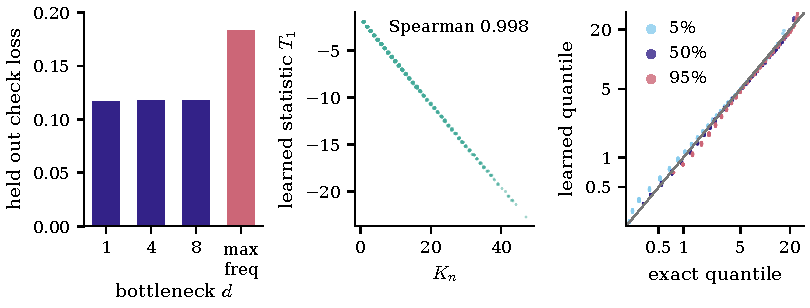
\includegraphics{figures/suff_gbc.pdf}
\caption{Infinite alleles model, $n=100$. Left: held out check loss at bottleneck dimensions
$1$, $4$ and $8$ and for the largest allele frequency alone; widening the bottleneck buys
nothing, while the nonsufficient summary is badly penalised. Centre: the learned one
dimensional statistic against $K_n$, Spearman $0.998$. Right: learned posterior quantiles at
levels $5\%$, $50\%$ and $95\%$ against the exact posterior quantiles, computed with no
likelihood evaluation.}
\label{suff:fig:gbc}
\end{figure}

Against the exact posterior of Section \ref{suff:sec:esfpost}, the median relative errors in
the learned $5,25,50,75,95$ per cent quantiles are $10.4\%$, $4.9\%$, $2.5\%$, $3.6\%$ and
$8.1\%$. The learned $90\%$ interval covers the truth in $82.9\%$ of held out replicates
against $89.8\%$ for the exact posterior, so at this training budget the method is
overconfident in the tails. We report this because it is the honest limitation: the centre
of the posterior is recovered accurately and the extreme quantiles are the hardest part of
the fit, which is what one would expect from a check loss with few observations at extreme
$u$. Section \ref{suff:sec:calib} diagnoses the cause and Section \ref{suff:sec:locscale}
repairs it in the fits that converge.

\subsection{Capacity control}
\label{suff:sec:capacity}

Remark \ref{suff:rem:caveats} concedes that a flat risk curve could reflect an optimiser which
failed to exploit the extra capacity rather than genuine sufficiency. The concession is
testable and we test it. In a separate set of runs of the same design, on the same training
data with an independent held out sample of $5{,}000$ pairs, each configuration fitted from
$20$ random seeds, holding $d=1$ and widening $\varphi$ and $g$ gave

\begin{center}
\begin{adjustbox}{max width=\textwidth}
\begin{tabular}{lccc}
\toprule
$d=1$, hidden width & 64 & 128 & 256 \\
\midrule
held out check loss, mean of $20$ seeds & $0.11688$ & $0.11695$ & $0.11746$ \\
standard deviation over seeds & $0.00047$ & $0.00037$ & $0.00155$ \\
\bottomrule
\end{tabular}
\end{adjustbox}
\end{center}

Quadrupling the width does not lower the risk at all; the widest network is if anything
slightly worse and less stable, and no difference in loss between widths has a $95\%$ Welch interval
that excludes zero. That is the signature of a budget which is not binding, not of capacity
starvation. The same runs at $d=4$ and $d=8$ give mean losses $0.11689$ and $0.11671$, so the
mean gaps among $d=1$, $4$ and $8$ are at most $0.0002$, again with intervals that include
zero, while single fits at $d=1$ range from $0.11632$ to $0.11813$. Run to run variation at a
fixed bottleneck is larger than the effect of the bottleneck.

This is what a genuine flat region looks like, and it is the control that Corollary
\ref{suff:cor:test} requires before a positive result may be believed. It also calibrates how
finely the risk curve can be read: at this training budget and with a single run per
configuration, differences below roughly $0.002$ should not be interpreted. The infinite
sites comparison of Section \ref{suff:sec:sites} therefore uses three random seeds per
configuration, and a separate study uses $50$, so that its smaller differences can be judged against their own spread.

\subsection{Calibration}
\label{suff:sec:calib}

Because the map is fitted, it can be miscalibrated, and because the joint law is available by
simulation, miscalibration can be measured exactly. The diagnostic is the one of
\citet{suff:cook2006}: if $H_\phi$ were the true posterior quantile function then for a
simulated pair $(\theta,y)$ the rank of $\theta$ under the fitted map, the $u$ with $H_\phi(u,y)=\theta$, would be uniform, so the proportion of
held out replicates with $\theta$ below the fitted $q$th quantile should equal $q$.

In the main run the fitted $90\%$ central interval covers in $82.9\%$ of held out replicates
against $89.8\%$ for the exact posterior. The centre is accurate, with a median relative error
of $2.5\%$ in the posterior median, and the error grows toward the tails, reaching $10.4\%$ at
the fifth percentile and $8.1\%$ at the ninety fifth. This is the expected failure mode for a
check loss: extreme $u$ are visited rarely during training and the corresponding quantiles are
estimated from correspondingly less information.

The obvious remedies do not work, and we report the fact because it locates the difficulty
correctly. In the second set of runs, with its independent held out sample and $20$ seeds per
configuration, tripling the number of training steps, and separately drawing $u$ from a
$\Be(1/2,1/2)$ proposal with importance reweighting so that extreme quantiles are visited far
more often, both left the coverage where it was (means over seeds):

\begin{center}
\begin{adjustbox}{max width=\textwidth}
\begin{tabular}{lcc}
\toprule
& coverage of nominal $90\%$ & held out check loss \\
\midrule
uniform $u$, $700$ steps            & $0.836$ & $0.11688$ \\
uniform $u$, $2100$ steps           & $0.838$ & $0.11621$ \\
tail weighted $u$, $2100$ steps     & $0.837$ & $0.11629$ \\
exact posterior                     & $0.893$ & $\cdot$ \\
\bottomrule
\end{tabular}
\end{adjustbox}
\end{center}

The mechanism is not undertraining but shrinkage of the extreme quantiles toward the centre.
In the main run the signed median relative errors are $+10.4\%$ at the fifth percentile and
$-7.4\%$ at the ninety fifth, so the errors point inward from both sides and the fitted $90\%$
interval is $0.86$ of the correct width. That is a bias in the fitted quantile function, of
the kind familiar from any smooth regression of a quantity that varies sharply with the
covariate, and it will not be removed by visiting the tails more often.

It also exposes a real limitation of Theorem \ref{suff:thm:quant}. The excess risk here is
small, so the theorem certifies that the fitted posterior is close to the exact one in $W_2$,
and it is. But $W_2$ integrates the quantile discrepancy uniformly in $u$, and a fourteen per
cent deficit in interval width contributes very little to it relative to the overall
posterior spread. Wasserstein closeness therefore controls the bulk of the posterior and is
nearly blind to tail calibration, as Example \ref{suff:ex:onegene3} anticipated. A small excess
risk is not a substitute for calibrating directly.

\subsection{A parametrisation that fixes it}
\label{suff:sec:locscale}

The diagnosis suggests the repair. If the difficulty is that extreme quantiles are regressed
toward the centre, the remedy is to arrange for them to be extrapolated rather than fitted.
Replace \eqref{suff:eq:deepsets} by
\begin{equation}
H(u,y)\;=\;\mu\big(T_\varphi(y)\big)\;+\;\exp\!\big\{\varsigma(T_\varphi(y))\big\}\,\Phi^{-1}(u)
\;+\;\eta\,c\big(\Phi^{-1}(u),\,T_\varphi(y)\big),
\label{suff:eq:locscale}
\end{equation}
with $\mu$, $\varsigma$, $\varphi$ and $c$ learned and $\eta$ a small fixed constant, taken
here as $0.3$. The quantile level enters through $\Phi^{-1}(u)$ inside an explicit location
scale term, so the map is exactly linear in $z=\Phi^{-1}(u)$ up to the correction $c$. It is
increasing in $u$, hence a legitimate quantile function, whenever
$\eta\,|\partial c/\partial z|<\exp\{\varsigma(T_\varphi(y))\}$ pointwise, a condition we
encourage by taking $\eta$ small. In the fits reported below the five fitted quantile levels stayed in order on every held out sample, but the condition did not hold everywhere: in $8$ of the $12$ converged fits $\partial H/\partial z$ turns negative somewhere in $|z|\le3.5$, so taking $\eta$ small does not by itself guarantee a monotone quantile function, and an application should constrain $c$ or check monotonicity on a grid as we did. Nothing else
changes: the loss is still \eqref{suff:eq:objective}, the bottleneck is still $T_\varphi$, and
Theorems \ref{suff:thm:suff} and \ref{suff:thm:quant} apply unaltered, since they constrain
only how the data enter. When $c\equiv0$ the family \eqref{suff:eq:locscale} contains the exact
answer of the Gaussian example of Section \ref{suff:sec:toy}, which is the reason to expect it
to extrapolate well.

On the same held out sample as the second set of runs, again with $20$ seeds, the fit is bimodal. In $8$ of the $20$ seeds the bottleneck never finds $K_n$ (Spearman correlation $0.94$ to $0.98$ rather than $0.998$), and the held out check loss, $0.128$ to $0.160$, is far worse than any plain fit; these failures are obvious from the loss alone, which is how one would screen them in practice. In the other $12$ the repair is complete. The table gives means over seeds, for the plain parametrisation at $2100$ steps and for the $12$ converged location scale fits.

\begin{center}
\begin{adjustbox}{max width=\textwidth}
\begin{tabular}{lccccc}
\toprule
& coverage & $5\%$ & $50\%$ & $95\%$ & width ratio \\
\midrule
plain, $u$ as input \eqref{suff:eq:deepsets} & $0.838$ & $+9.4\%$ & $+0.2\%$ & $-8.4\%$ & $0.86$ \\
location scale \eqref{suff:eq:locscale}      & $0.899$ & $-1.8\%$  & $+0.6\%$ & $+0.7\%$ & $1.02$ \\
exact posterior                          & $0.893$ & $\cdot$ & $\cdot$ & $\cdot$ & $1.00$ \\
\bottomrule
\end{tabular}
\end{adjustbox}
\end{center}

Coverage moves from $0.838$ to $0.899$ against the exact posterior's $0.893$ on the same held
out sample. The signed errors at the fifth and ninety fifth percentiles fall from $+9.4\%$
and $-8.4\%$ to $-1.8\%$ and $+0.7\%$, and, decisively, they no longer point inward from both
sides, so the systematic narrowing is gone and the width ratio is $1.02$. The held out check
loss also improves, from $0.11621$ to $0.11546$, and every converged fit, between $0.11527$ and
$0.11568$, beats every plain fit of the second set of runs, which is the best we report on
this problem; the parametrisation is not buying calibration at the expense of accuracy.

We draw two lessons. The narrow one is that \eqref{suff:eq:locscale} should be the default
architecture for this class of problem, fitted from several seeds and screened by held out
loss, and that the cost of the plain parametrisation is paid entirely in the tails where it is
least visible. The broader one concerns what the
theory does and does not certify. Theorem \ref{suff:thm:quant} was satisfied by both rows of
the table, since both have small excess risk, and it was the direct calibration check rather
than the certificate that distinguished them. A generative posterior must be calibrated before
it is believed, in a way that an exact posterior need not be, and the diagnostic is cheap
because it uses simulations one has already generated.

\section{Worked example 2: the infinite sites model}
\label{suff:sec:sites}

This section applies the same test where the classical summary is not sufficient. We first
prove that it is not, by an explicit calculation, then compute its exact law, and finally
measure what discarding the rest of the data costs.

\subsection{Watterson's $S$ is not sufficient}

Consider $n$ sequences under the standard coalescent (Chapter~\ref{ch:coal}) with the
infinite sites mutation model at scaled rate $\theta$, and suppose the ancestral state at each
site is known. While there are $k$ lineages the waiting time to the next coalescence is
$T_k\sim\mathrm{Exp}\{k(k-1)/2\}$, independently for $k=n,\dots,2$ and independently of the
tree topology. Let $\ell_i$ be the total length of branches subtending exactly $i$ leaves,
$i=1,\dots,n-1$, let $L=\sum_i \ell_i=\sum_{k=2}^n kT_k$ be the total tree length, let
$\xi=(\xi_1,\dots,\xi_{n-1})$ be the site frequency spectrum, so that $\xi_i$ is the number of
sites at which the derived allele is carried by exactly $i$ sequences, and let
$S=\sum_i\xi_i$ be the number of segregating sites. Write
$a_n=\sum_{j=1}^{n-1}j^{-1}$ and $b_n=\sum_{j=1}^{n-1}j^{-2}$.

Before the proposition, the intuition. Given the tree, mutations fall on it as a Poisson
process, so the spectrum given $S$ and the tree is multinomial with probabilities $\ell/L$,
free of $\theta$. But the tree is not observed, and the number of mutations $S$ is
informative about the tree length $L$ in a way that depends on $\theta$: for the same $S$, a
small $\theta$ suggests a long tree and a large $\theta$ a short one. Long trees and short
trees have different shapes, so the conditional law of the spectrum given $S$ depends on
$\theta$ through this back door. The proposition makes the back door explicit at $S=1$.

\begin{proposition}
\label{suff:prop:notsuff}
Conditionally on the coalescent tree, $\xi_i\sim \mathrm{Poisson}(\theta\ell_i/2)$
independently, so that $S\sim\mathrm{Poisson}(\theta L/2)$ and
$\xi\mid S,\mathrm{tree} \sim \mathrm{Multinomial}(S;\ \ell/L)$, free of $\theta$.
Unconditionally, let $e_{n-1}$ be the spectrum with a single site carried by $n-1$
sequences, and
\[
\phi_n(\theta)=\Prob(\xi=e_{n-1}\mid S=1,\theta)
=\frac{\E\big[\ell_{n-1}e^{-\theta L/2}\big]}{\E\big[L\,e^{-\theta L/2}\big]} .
\]
Then for $n\ge3$, $\phi_n(0+)=1/\{(n-1)a_n\}$ and
\[
\phi_n'(0+)=-\,\frac{a_n-b_n}{(n-1)\,a_n^{2}}<0 .
\]
In particular $\phi_n$ is not constant in $\theta$, and $S$ is not sufficient for $\theta$.
\end{proposition}

\begin{proof}
Given the tree, $\Prob(\xi=e_{n-1}\mid\mathrm{tree})=(\theta\ell_{n-1}/2)e^{-\theta L/2}$ and
$\Prob(S=1\mid\mathrm{tree})=(\theta L/2)e^{-\theta L/2}$; averaging over the tree and dividing
gives the formula for $\phi_n$. Branches subtending $n-1$ leaves exist only while two lineages
remain, and one of the two does so exactly when the root split is $\{1,n-1\}$. Under the
coalescent the size of one side of the root split is uniform on $\{1,\dots,n-1\}$
\citep{suff:kingman1982}, so $\ell_{n-1}=NT_2$ with $N$ an indicator independent of the
$T_k$ and $\E N=2/(n-1)$. With $\E T_k=2/\{k(k-1)\}$, $\E T_2^2=2$ and the independence of the
$T_k$,
\[
\E\ell_{n-1}=\frac{2}{n-1},\qquad
\E[\ell_{n-1}L]=\frac{2}{n-1}\Big(2\E T_2^2+\sum_{k=3}^{n}k\,\E T_k\Big)
=\frac{2}{n-1}\,(2+2a_n),
\]
and $\E L=2a_n$, $\Var L=\sum_k k^2\Var T_k=4b_n$, so $\E L^2=4b_n+4a_n^2$. The functions
$\lambda\mapsto\E[\ell_{n-1}e^{-\lambda L}]$ and $\lambda\mapsto\E[Le^{-\lambda L}]$ are
differentiable at $\lambda=0$ from the right because $L$ has all moments. Hence, with
$\lambda=\theta/2$, $\phi_n(0+)=\E\ell_{n-1}/\E L=1/\{(n-1)a_n\}$ and
\begin{align*}
\frac{\dd\phi_n}{\dd\lambda}\Big|_{0+}
&=\frac{\E\ell_{n-1}}{\E L}\Big\{\frac{\E L^2}{\E L}-\frac{\E[\ell_{n-1}L]}{\E\ell_{n-1}}\Big\}\\
&=\frac{1}{(n-1)a_n}\Big\{2a_n+\frac{2b_n}{a_n}-2-2a_n\Big\}
=-\frac{2(a_n-b_n)}{(n-1)a_n^2}.
\end{align*}
Dividing by two gives $\phi_n'(0+)$, which is negative because $1/j^2<1/j$ for $j\ge2$, so
$a_n>b_n$ when $n\ge3$. A function with nonzero right derivative at $0$ takes different values
at two points of $(0,\infty)$. Sufficiency of $S$ would require the conditional law of $\xi$
given $S=1$, an event of positive probability, to be the same for all $\theta$, which fails.
\end{proof}

The genetic content of Proposition \ref{suff:prop:notsuff} is that the \emph{shape} of the
spectrum carries information about the total tree length, which in turn carries information
about $\theta$. A lone variant carried by all but one sequence sits on a root branch, and
root branches are long precisely in long trees; as $\theta$ grows, the trees compatible with a
single mutation get shorter, and the chance that the mutation sits on a root branch falls.
This is why Watterson's estimator is known to be inefficient relative to the full data
likelihood \citep{suff:felsenstein1992,suff:fuli1993}. What the generative framework adds is
that the loss can now be measured rather than argued.

\begin{example}[Three sequences]
\label{suff:ex:three}
For $n=3$ everything is explicit. The spectrum is $(\xi_1,\xi_2)$, with $\ell_1=3T_3+T_2$ and
$\ell_2=T_2$, where $T_3\sim\mathrm{Exp}(3)$ and $T_2\sim\mathrm{Exp}(1)$. Integrating the
Poisson probabilities against these exponentials gives rational functions of $\theta$; for
example
\[
\Prob(\xi=(0,1)\mid\theta)=\frac{\theta}{(\theta+1)^2(\theta+2)},\qquad
\Prob(\xi=(1,0)\mid\theta)=\frac{\theta(3\theta+4)}{(\theta+1)^2(\theta+2)^2},
\]
whose sum is $\Prob(S=1\mid\theta)=2\theta(2\theta+3)/\{(\theta+1)^2(\theta+2)^2\}$, in agreement
with Proposition \ref{suff:prop:Slaw} below. The first of these takes one line:
$\E[(\lambda T_2)e^{-3\lambda T_3-2\lambda T_2}]=\lambda(1+\lambda)^{-1}(1+2\lambda)^{-2}$ with
$\lambda=\theta/2$. Hence
\[
\phi_3(\theta)=\Prob(\xi=(0,1)\mid S=1,\theta)=\frac{\theta+2}{2(2\theta+3)},
\]
which decreases from $1/3$ at $\theta=0$ to $1/4$ as $\theta\to\infty$, with slope $-1/18$ at
the origin, as Proposition \ref{suff:prop:notsuff} predicts since $a_3=3/2$ and $b_3=5/4$. A
simulation of $4\times10^5$ coalescent trees gives $0.322$ at $\theta=0.2$ and $0.279$ at
$\theta=3$, against the exact $0.324$ and $0.278$.

The failure is visible in likelihood ratios. Two data sets with the same $S=1$, a singleton
and a doubleton, have likelihood ratio
\[
\frac{\Prob(\xi=(0,1)\mid\theta)}{\Prob(\xi=(1,0)\mid\theta)}=\frac{\theta+2}{3\theta+4},
\]
which is $0.43$ at $\theta=1$ and $0.375$ at $\theta=4$; a sufficient $S$ would make it
constant. With $S=2$ the three possible spectra give
\[
\frac{L(1)}{L(4)}=\frac{4625}{3136}=1.47,\qquad \frac{625}{352}=1.78,\qquad
\frac{125}{64}=1.95
\]
for $(2,0)$, $(1,1)$ and $(0,2)$ respectively. Two doubletons, both mutations on the internal
branch, favour small $\theta$ most strongly, because they point to a long internal branch and
hence a long tree. Under the log uniform prior on $[0.5,30]$ used in Section
\ref{suff:sec:simsites}, the posterior medians given the full spectrum are $1.83$, $1.66$ and
$1.58$, against $1.73$ given $S=2$ alone. The differences are modest at $n=3$, where the
spectrum has only two cells, and grow with $n$ as the shape of the spectrum becomes more
informative about the tree.
\end{example}

\subsection{What the second coordinate is}
\label{suff:sec:secondcoord}

Proposition \ref{suff:prop:notsuff} says a second number is needed; it does not say which. The
fitted map answers that question empirically, and the answer is recognisable.

Write $\pi_{\mathrm{T}}=\binom{n}{2}^{-1}\sum_{i=1}^{n-1}i(n-i)\xi_i$ for the mean pairwise
difference and recall Tajima's $D$ \citep{suff:tajima1989}, which contrasts $\pi_{\mathrm{T}}$
with $S/a_n$, standardised by an estimate of the standard deviation of the difference. On held
out data the two learned coordinates $(T_1,T_2)$ of the $d=2$ fit (not the waiting times $T_k$ above) divide the labour cleanly.
The coordinate $T_2$ carries the overall mutation count, with absolute Spearman correlations
$0.988$ with $S$ and $0.944$ with $\pi_{\mathrm{T}}$. The coordinate $T_1$ is almost
uncorrelated with both, at $0.04$ and $0.12$; it is not a measure of how many mutations there
are. Figure \ref{suff:fig:p2} shows the split: colour, which is $\log\theta$, changes along
$T_2$ and hardly at all along $T_1$.

What then is $T_1$? Regressing each learned coordinate on a cubic in the separately fitted
$d=1$ scalar, which is itself a near monotone function of $S$, and correlating the residual
with $D$ gives absolute correlations $0.73$ for $T_1$ and $0.44$ for $T_2$. The coordinate that
carries no count information is, to a substantial degree, a spectrum shape contrast of
Tajima's kind, which is what Proposition \ref{suff:prop:notsuff} predicts, since the shape of
the spectrum is what carries information about the total tree length.

We read this cautiously. The correlation with $D$ is substantial but not close to one, and
under strict neutrality $D$ has mean near zero by construction, so there is limited shape
variation for the network to exploit. The clean test of the idea is the one described in
Section \ref{suff:sec:ext}: run the same procedure under selection, where $D$ has genuine
signal, and see whether the learned second coordinate tracks it. That experiment is not in
this chapter.

\subsection{The exact law of the number of segregating sites}
\label{suff:sec:Slaw}

To quantify what $S$ discards we need the exact posterior given $S$, which is available
through a classical representation due to \citet{suff:watterson1975}.

\begin{proposition}
\label{suff:prop:Slaw}
Under the standard coalescent with infinite sites mutation at scaled rate $\theta$,
\[
S \;\stackrel{d}{=}\; \sum_{j=1}^{n-1}G_j,
\qquad G_j \ \text{independent},\quad
\Prob(G_j=k)=\Big(\frac{\theta}{\theta+j}\Big)^{k}\frac{j}{\theta+j},\ k\ge0 .
\]
Consequently $\E S=\theta a_n$, which is Watterson's estimating equation, and
$\Var S=\theta a_n+\theta^2 b_n$.
\end{proposition}

\begin{proof}
While the ancestral process has $k$ lineages, mutations arrive at total rate $k\theta/2$ and
coalescences at rate $k(k-1)/2$, as independent Poisson processes. By the competing
exponentials property, each successive event is a mutation with probability
$(k\theta/2)/\{k\theta/2+k(k-1)/2\}=\theta/(\theta+k-1)$, independently of everything before,
until the first coalescence ends the phase. The number of mutations occurring while there are
$k$ lineages is thus geometric on $\{0,1,\dots\}$ with success probability
$(k-1)/(\theta+k-1)$, and the phases are independent by the strong Markov property. Writing
$j=k-1$ and summing over $k=2,\dots,n$ gives the display. A geometric variable with success
probability $j/(\theta+j)$ has mean $\theta/j$ and variance $\theta/j+\theta^2/j^2$, and the
moments of $S$ follow by summation.
\end{proof}

The probability generating function is the product
$\E z^S=\prod_{j=1}^{n-1}j/(j+\theta-\theta z)$, so the law of $S$ is a convolution of $n-1$
geometric mass functions and $\pi(\theta\mid S)$ can be computed to machine precision on a
grid or by adaptive quadrature. This is what we use as the comparison in Table
\ref{suff:tab:abc} and Figure \ref{suff:fig:p2}. The proposition also explains why $S$ is a
natural summary: it has a clean law, and Watterson's estimator $S/a_n$ falls out of it.
Proposition \ref{suff:prop:notsuff} says that naturalness is not sufficiency.

\begin{example}[The law of $S$ for five sequences]
\label{suff:ex:five}
For $n=5$, $S=G_1+G_2+G_3+G_4$ with success probabilities $j/(\theta+j)$, $a_5=25/12$ and
$b_5=205/144$. Two values are immediate from the generating function:
\[
\Prob(S=0\mid\theta)=\prod_{j=1}^{4}\frac{j}{\theta+j},\qquad
\Prob(S=1\mid\theta)=\Prob(S=0\mid\theta)\sum_{j=1}^{4}\frac{\theta}{\theta+j},
\]
so at $\theta=1$ these are $24/120=1/5$ and $\tfrac15\cdot\tfrac{77}{60}=77/300=0.2567$. The
full mass functions at $\theta=1$ and $\theta=3$, obtained by convolving the four geometric
laws, are
\begin{center}
\begin{adjustbox}{max width=\textwidth}
\begin{tabular}{lcccccccccc}
\toprule
$s$ & 0 & 1 & 2 & 3 & 4 & 5 & 6 & 7 & 8 & $\ge9$ \\
\midrule
$\theta=1$ & 0.2000 & 0.2567 & 0.2111 & 0.1423 & 0.0861 & 0.0487 & 0.0264 & 0.0140 & 0.0072 & 0.0075 \\
$\theta=3$ & 0.0286 & 0.0651 & 0.0935 & 0.1085 & 0.1111 & 0.1049 & 0.0937 & 0.0804 & 0.0670 & 0.2472 \\
\bottomrule
\end{tabular}
\end{adjustbox}
\end{center}
with means $25/12=2.083$ and $25/4=6.25$ and variances $3.507$ and $19.06$, exactly as the
proposition gives. A simulation of $4\times10^5$ coalescent trees with Poisson mutations
reproduces every entry to within $0.002$. The variance at $\theta=3$ is three times the mean,
not equal to it as a Poisson count would be: the extra term $\theta^2b_n$ is the randomness of
the tree, and it is the reason a single locus is so uninformative. Under the log uniform
prior on $[0.5,30]$ the posterior given $S=3$ has median $1.62$ and $90\%$ interval
$(0.60,\,5.91)$, a tenfold range, against Watterson's estimate $3/a_5=1.44$.
\end{example}

\subsection{Numerical results}
\label{suff:sec:simsites}

We simulate $n=30$ sequences, $M=30{,}000$ training replicates, $\theta$ log uniform on
$[0.5,30]$, using exact coalescent simulation with branch wise Poisson mutation. The input to
\eqref{suff:eq:deepsets} is the raw spectrum as the set $\{(i,\xi_i)\}$. We also fit a
baseline that sees only $S$, and we compute the exact posterior $\pi(\theta\mid S)$ from
Proposition \ref{suff:prop:Slaw}. Because the differences to be resolved here are smaller than
in Section \ref{suff:sec:esf}, every configuration is fitted from three random seeds.

\begin{table}[t]
\centering
\begin{adjustbox}{max width=\textwidth}
\begin{tabular}{lcccc}
\toprule
& $S$ only & $d=1$ & $d=2$ & $d=4$ \\
\midrule
held out check loss, mean of three seeds & 0.10550 & 0.09834 & 0.09831 & 0.09748 \\
range over seeds & 0.10540 to 0.10565 & 0.09823 to 0.09850 & 0.09730 to 0.09889 & 0.09712 to 0.09776 \\
\bottomrule
\end{tabular}
\end{adjustbox}
\caption{Infinite sites model, $n=30$. Unlike Table \ref{suff:tab:esf}, the risk falls as the
bottleneck widens from $d=1$ to $d=4$, and a rerun with $50$ seeds per configuration puts the
gap between them clear of zero, so by Corollary \ref{suff:cor:test} no one dimensional statistic of the kind the
network represents is sufficient. The learned scalar at $d=1$ also beats Watterson's $S$
by a wide margin: even among one dimensional summaries, $S$ is not the best.}
\label{suff:tab:sites}
\end{table}

Two things in Table \ref{suff:tab:sites} are worth separating. The gap of $0.0072$ between the
$S$ only column and $d=1$ says that $S$ is not the best scalar summary. The gap of $0.0009$
between $d=1$ and $d=4$ says that no scalar summary in the class suffices, a wider statement than Proposition \ref{suff:prop:notsuff}, which concerns $S$ alone, and one detected here by fitting; it is small, and three seeds alone cannot settle it, so we refitted every configuration from $50$ seeds on the same simulated data. The mean gap between $d=1$ and $d=4$ is then $0.00088$, with $95\%$ Welch interval $(0.00068,\,0.00107)$, and $d=2$ sits between, $0.00040$ below $d=1$ and $0.00047$ above $d=4$, each with an interval that excludes zero. Single fits still overlap: a $d=1$ fit beats a $d=4$ fit in about one pair in ten, which is why one run per configuration cannot resolve a difference of this size. The seeds vary only the training randomness, not the simulated data, so the interval measures optimisation noise at this training budget, and the reading rests on the fitted class, not on a proof.
The learned scalar at $d=1$ has Spearman correlation $0.991$ with $S$ in absolute value, so it
is a reweighted count of segregating sites rather than something exotic.

In posterior terms the loss is substantial. Over 500 held out datasets the median width of the
$90\%$ interval, divided by the true $\theta$, is $0.980$ using the whole spectrum against
$1.294$ using the exact posterior given $S$ alone, a reduction of $24\%$. On the same datasets
the generative interval covers the truth in $85.8\%$ of cases against $92.0\%$ for the exact
posterior given $S$, so part of the narrowing is the tail shrinkage diagnosed in Section
\ref{suff:sec:calib}, which in Section \ref{suff:sec:esf} cost about $14\%$ of width. The
remainder, roughly ten per cent of the interval, is information in the shape of the spectrum
that $S$ throws away, and the location scale parametrisation of Section \ref{suff:sec:locscale}
would be used in any application to separate the two cleanly. Discarding the shape of the
spectrum in favour of its total is not a harmless simplification.

\begin{figure}[t]
\centering
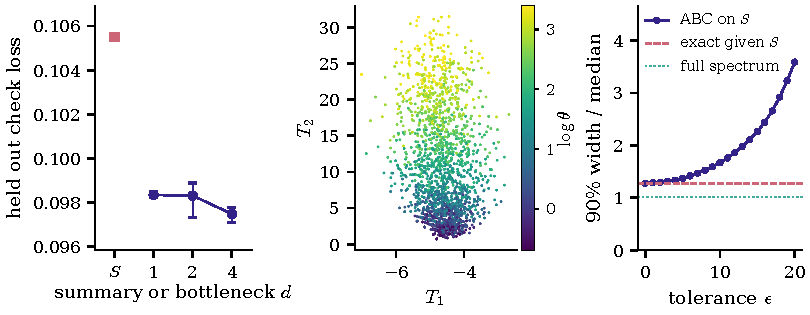
\includegraphics{figures/suff_p2.pdf}
\caption{Infinite sites model, $n=30$. Left: held out check loss for $S$ alone and for
bottlenecks $d=1,2,4$, mean and range over three seeds; unlike the infinite alleles case,
widening the bottleneck continues to help, so no scalar summary in the class suffices, a wider statement than Proposition \ref{suff:prop:notsuff}, which concerns $S$ alone. Centre: the learned two dimensional bottleneck on held out data, coloured
by $\log\theta$; $T_2$ carries the mutation count and $T_1$ the shape of the spectrum. Right:
for the observed dataset of Section \ref{suff:sec:eff}, the ABC posterior width, $90\%$
interval divided by median, as a function of tolerance, against the exact posterior given $S$
(width $1.27$) and the generative posterior using the whole spectrum (width $1.02$).}
\label{suff:fig:p2}
\end{figure}

\subsection{The two examples read together}
\label{suff:sec:together2}

The two worked examples are chosen to be a matched pair, and the contrast between Tables
\ref{suff:tab:esf} and \ref{suff:tab:sites} is the empirical core of the chapter.

In both cases the same kind of architecture, the same loss and the same protocol are applied,
and the only thing varied is the bottleneck dimension. In the infinite alleles model the risk
curve is flat from $d=1$: the values $0.1164$, $0.1178$ and $0.1175$ at $d=1,4,8$ differ by
less than the run to run variation, so by Corollary \ref{suff:cor:minimal} we read
$d^\star=1$. In the infinite sites model the curve is still falling at $d=4$, from $0.0983$ to
$0.0975$, by a gap whose interval over $50$ seeds excludes zero, so $d^\star>1$.

That contrast is the whole diagnostic, and it is worth being clear about what makes it
credible. If the procedure reported $d^\star=1$ everywhere, it would be uninformative. If it
reported $d^\star>1$ everywhere, it would be detecting optimisation failure rather than
insufficiency. It reports $d^\star=1$ where \citet{suff:ewens1972} proves that it should and
$d^\star>1$ where Proposition \ref{suff:prop:notsuff} proves that $S$ fails, with no tuning
between the two runs. The scalar it finds in the first case is $K_n$, to Spearman $0.998$.

The second half of the argument is that the excess risk is not merely detectable but
material. A $56\%$ excess for the largest allele frequency summary, a choice an ABC analyst
might plausibly have made, corresponds to discarding most of the information. Watterson's $S$
is a far better summary, chosen for good reasons and supported by Proposition
\ref{suff:prop:Slaw}, and it still costs a substantial part of the posterior interval. The
lesson is not that summaries are useless but that their cost is invisible unless something
like Corollary \ref{suff:cor:minimal} is computed, and that a well motivated summary can still
be expensive.

\section{Efficiency}
\label{suff:sec:eff}

This section compares rejection ABC and the generative fit on one dataset, then on many. We
use the infinite sites problem of Section \ref{suff:sec:simsites} with an observed dataset
simulated at $\theta=8$, and give ABC the benefit of the best simple scalar, $S$ itself.

\begin{example}[One simulated locus]
\label{suff:ex:locus}
The observed sample, a clearly labelled simulation rather than real data, has $n=30$ sequences
and $S=23$ segregating sites, with spectrum
\[
\xi_1=4,\quad \xi_2=1,\quad \xi_3=3,\quad \xi_7=7,\quad \xi_{17}=1,\quad \xi_{20}=1,\quad
\xi_{23}=6,
\]
and all other $\xi_i=0$. Watterson's estimate is $23/a_{30}=23/3.962=5.81$, the mean pairwise
difference is $\pi_{\mathrm{T}}=6.73$, and Tajima's $D=0.56$. Under the log uniform prior on
$[0.5,30]$ the exact posterior given $S=23$, computed from Proposition \ref{suff:prop:Slaw} by
adaptive quadrature, has median $6.00$, mean $6.37$ and $90\%$ interval $(3.19,\,10.81)$, so
its relative width, the interval length divided by the median, is $1.269$; the maximum
likelihood estimate from $S$ alone is $6.11$.

The spectrum has a striking shape. Thirteen of the $23$ variants sit at frequencies $7/30$
and $23/30$, which are complementary: they are the mutations on the two branches below the
root of a genealogy whose first split separates seven sequences from twenty three. So many
mutations on the root branches say that those branches are long, hence that the tree is long,
hence that $23$ mutations reflect a smaller $\theta$ than a typical tree would suggest. This
is Proposition \ref{suff:prop:notsuff} at work on a single dataset, and the generative
posterior using the whole spectrum duly moves down, to a median of $4.76$, with relative width
$1.02$. Here the move is away from the true value $8$, which is a reminder that one
dataset proves nothing either way: what matters is calibration over many datasets, which the
previous section measured.
\end{example}

Table \ref{suff:tab:abc} shows rejection ABC on this dataset, with $2\times10^5$ prior draws
and acceptance when $|S_{\mathrm{sim}}-23|\le\epsilon$. Since the ABC target
\eqref{suff:eq:abctarget} depends only on the law of $S$, it can also be computed exactly, and
the table gives both. At $\epsilon=0$ rejection ABC samples exactly from $\pi(\theta\mid S=23)$,
so its median, $5.96$ from $2{,}094$ draws, agrees with the exact $6.00$ to within Monte Carlo
error, whose standard deviation is about $0.06$.

\begin{table}[t]
\centering
\begin{adjustbox}{max width=\textwidth}
\begin{tabular}{lrrrrr}
\toprule
tolerance $\epsilon$ & 0 & 2 & 5 & 10 & 20 \\
\midrule
\multicolumn{6}{l}{\emph{rejection ABC, $2\times10^5$ simulations}} \\
acceptance rate           & 1.05\% & 5.39\% & 11.9\% & 24.1\% & 65.6\% \\
accepted draws            & 2094 & 10773 & 23815 & 48232 & 131153 \\
posterior median          & 5.96 & 5.94 & 5.82 & 5.36 & 3.02 \\
relative posterior width  & 1.275 & 1.293 & 1.372 & 1.669 & 3.586 \\
\midrule
\multicolumn{6}{l}{\emph{exact ABC target \eqref{suff:eq:abctarget}}} \\
acceptance probability    & 1.06\% & 5.33\% & 11.9\% & 24.1\% & 65.6\% \\
posterior median          & 6.00 & 5.97 & 5.84 & 5.37 & 3.00 \\
relative posterior width  & 1.269 & 1.290 & 1.374 & 1.668 & 3.614 \\
\bottomrule
\end{tabular}
\end{adjustbox}
\caption{Rejection ABC for the simulated locus of Example \ref{suff:ex:locus}, true
$\theta=8$, observed $S=23$, prior log uniform on $[0.5,30]$. Relative width is the $90\%$
interval length divided by the median. At $\epsilon=0$ the target is the exact
$\pi(\theta\mid S=23)$, with median $6.00$ and relative width $1.269$; the Monte Carlo values
agree with it to within sampling error. Tolerance buys acceptance and pays in bias: at
$\epsilon=20$ the posterior has collapsed towards the prior, whose median is $3.87$.}
\label{suff:tab:abc}
\end{table}

The bias of tolerance in Table \ref{suff:tab:abc} is the finite tolerance counterpart of the bias of Proposition
\ref{suff:prop:d2}: the Monte Carlo and exact rows agree, so none of the drift is sampling
error. Up to $\epsilon=5$ the median moves by less than three per cent while the acceptance
rate rises elevenfold; beyond that the drift accelerates, and at $\epsilon=20$ the median has
halved.

The arithmetic of D4 is the decisive point. ABC at $\epsilon=0$ required $2\times10^5$
simulations to produce about $2{,}100$ draws for a single dataset. The generative fit used
$3\times10^4$ simulations in total and thereafter returns posterior draws for any dataset at
the cost of a single evaluation. For a study with $10^4$ independent loci and rejection ABC with fresh simulations for each locus, the comparison is
approximately $1.9\times10^9$ simulations against $3\times10^4$, a factor of about
$6\times10^4$, and the generative posterior conditions on the whole spectrum while the ABC
posterior conditions on $S$.

\subsection{The genome scale comparison}

Proposition \ref{suff:prop:d4} becomes vivid when the number of datasets is realistic. A modern
study analyses each of many loci, or each of many windows along a genome, under a common
model. Writing $R$ for that count and taking the measured $\alpha_0=1.05\times10^{-2}$ and a
target of $n_{\mathrm{eff}}=2\times10^3$ draws per locus, for rejection ABC with fresh simulations for each locus:

\begin{center}
\begin{adjustbox}{max width=\textwidth}
\begin{tabular}{lrrrr}
\toprule
number of loci $R$ & 1 & $10^2$ & $10^4$ & $10^6$ \\
\midrule
rejection ABC simulations & $1.9\times10^5$ & $1.9\times10^7$ & $1.9\times10^9$ &
$1.9\times10^{11}$ \\
generative simulations & $3\times10^4$ & $3\times10^4$ & $3\times10^4$ & $3\times10^4$ \\
ratio & $6.3$ & $6.3\times10^{2}$ & $6.3\times10^{4}$ & $6.3\times10^{6}$ \\
\bottomrule
\end{tabular}
\end{adjustbox}
\end{center}

Two qualifications. The generative row assumes a common sample size across loci, and the
caveat of Section \ref{suff:sec:ext} about varying $n$ applies; training across a range of $n$
raises $M$ by a modest factor, not by a factor of $R$. And the comparison is against rejection
ABC; sequential methods reduce the ABC row, though they do not amortise it, since each new
dataset restarts the sequence. A table of simulated pairs shared across loci avoids the linear growth of the ABC row, since its size is set by the locus with the smallest acceptance probability.

The more important point is not the ratio but what is being purchased. The ABC column buys
$R$ posteriors conditioned on $S$; the generative column buys $R$ posteriors conditioned on
the whole configuration, which by Section \ref{suff:sec:sites} are materially narrower. The
method is simultaneously cheaper and conditioning on more.

\section{Extensions and limitations}
\label{suff:sec:ext}

This section records where the method should be taken next and where it is weakest.

\subsection{Where the programme goes next}

The two examples were chosen because in one the answer is known and in the other it can be
computed. Neither is where the method is needed. Three targets follow immediately.

\paragraph{The ancestral recombination graph.} With recombination the data is a collection of
correlated genealogies and the likelihood is intractable in a stronger sense than under the
infinite sites model, since even the one dimensional summaries lack closed form laws. The
architecture of Section \ref{suff:sec:arch} extends by treating the data as a set of site
patterns with position features, and the bottleneck test of Corollary \ref{suff:cor:test}
applies unchanged. The interesting output is not the posterior for the recombination rate,
which several methods already estimate, but the dimension at which the held out risk stops
falling, which is an estimate of how many numbers a recombining sample is worth.

\paragraph{Selection.} Under directional or balancing selection the genealogy is no longer the
neutral coalescent and the frequency spectrum is distorted in ways that Tajima's $D$ and its
relatives are designed to detect. Those statistics are hand built two dimensional summaries.
The framework here fits the analogous object rather than positing it, and the comparison
between the learned two dimensional bottleneck and the pair $(S,\pi_{\mathrm{T}})$ is a direct
test of how much the classical construction leaves on the table.

\paragraph{Multiple merger coalescents.} For $\Lambda$ coalescents the sufficiency question is
genuinely open and the simulation is straightforward, which is the combination the method
wants. Here the bottleneck dimension is itself the scientific quantity: it says how many
independent features of the spectrum distinguish a multiple merger history from a neutral
one.

\subsection{Limitations}

\paragraph{The test is a comparison of fits, not a proof.} Corollary \ref{suff:cor:test}
concerns population risks; we compare held out empirical risks. A negative result, meaning
that the risk keeps falling as $d$ grows, is the safer of the two, since it exhibits an actual
improvement. A positive result, meaning that widening the bottleneck buys nothing, is weaker:
it could reflect an optimiser that failed to exploit the extra capacity. The remedy is the
one adopted in Section \ref{suff:sec:arch}, holding the architecture and budget fixed and
varying only $d$, and then checking that increasing capacity at fixed $d$ does not help
either. Section \ref{suff:sec:capacity} carries out that check. And, as Remark
\ref{suff:rem:dimension} explains, the dimension measured is relative to what the network can
represent.

\paragraph{Sufficiency is relative to the simulation prior.} Theorem \ref{suff:thm:suff}
delivers Bayes sufficiency with respect to the prior used to generate training data, and the
passage to classical sufficiency requires that prior to have full support. A prior
concentrated on a narrow range of $\theta$ can make an insufficient statistic appear
sufficient, because within that range there is little for the discarded information to
distinguish. Example \ref{suff:ex:three} shows the mechanism: the likelihood ratio between two
spectra with the same $S$ changes only from $0.45$ to $0.33$ as $\theta$ runs from $0.5$ to
infinity, so a prior on a short interval would barely see it. The prior range must therefore
be reported, and it should be wider than the range of scientific interest.

\paragraph{Amortisation assumes a fixed sample size and design.} The trained map takes inputs
of a fixed shape. Datasets with different $n$ require either retraining, or an architecture
that takes $n$ as an additional input and is trained across a range of $n$. The latter is
straightforward and is what one would do in practice, but it consumes part of the efficiency
advantage claimed in Proposition \ref{suff:prop:d4}.

\paragraph{Model misspecification is untouched.} Everything here conditions on the simulator
being correct. If the coalescent with the assumed demography is wrong, the generative
posterior is confidently wrong, and it is arguably more confidently wrong than ABC, since it
does not have a tolerance that inadvertently widens the answer. The check on this is
predictive: simulate from the fitted posterior and compare the implied spectra with the
observed one.

\paragraph{We compare against rejection ABC.} Table \ref{suff:tab:abc} uses plain rejection
ABC. Regression adjustment, ABC MCMC and sequential Monte Carlo variants all improve on it, in
some cases substantially, and a full comparison would include them. Our defence is that all
of them inherit Proposition \ref{suff:prop:d1} unchanged, since none of them alters the
summary, and Proposition \ref{suff:prop:d1} is the defect we are addressing.

\section{Connection to effective sample size}
\label{suff:sec:ess}

There is a second bridge to the companion literature which is worth recording, because it
runs in the opposite direction to everything above: from genetics to computation.

\citet{suff:ewenshossjer2025} show that the inbreeding, variance and eigenvalue effective
population sizes are three distinct functionals of a transition kernel. Read as statistics
rather than as genetics they are three familiar objects. The inbreeding size
$N_e^{(i)}=(2\pi_2)^{-1}$, where $\pi_2$ is the probability that two genes descend from a
common parent gene, counts identity by descent and is Kish's effective sample size. The
variance size $N_e^{(v)}=x(1-x)/(2V)$, for allele frequency $x$ and one generation variance
$V$ of its change, is asymptotic variance efficiency. The eigenvalue size
$N_e^{(e)}=\tfrac12(1-\lambda_{\max})^{-1}$ is the reciprocal spectral gap, that is the
relaxation time, which in Markov chain Monte Carlo governs the integrated autocorrelation time.

Their Table 2, in which $N_e^{(i)}$ over $k$ generations converges to $N_e^{(e)}$, is then the burn in theorem. We reproduce it from the spectral representation of their Equation (42). For the brother sister case $N_m=N_f=1$ the values at $k=1,2,5,10,20,50$ are $3.0000$, $2.7247$, $2.6672$, $2.6421$, $2.6300$, $2.6228$, converging to $N_e^{(e)}=2.6180$. These values approach the limit like $1/k$, with excess about $0.24/k$, because each averages over the initial transient. The geometric rate $|\lambda_2/\lambda_1|=0.382$, which more than halves the error per generation, governs instead the convergence to $\lambda_1$ of the ratio of the probabilities of not yet being identical by descent at consecutive generations. For $(N_m,N_f)=(2,20)$ that rate is $0.078$.

\citet{suff:thompson2013} develops the identity by descent calculus underlying the first of
these in detail, and it is the same quantity $\pi_2$ that appears in the definition of
$N_e^{(i)}$.

The relevance here is methodological. The generative posterior of Section \ref{suff:sec:gbc}
produces independent draws by construction, since each draw uses a fresh $u$, so its
effective sample size equals its nominal one. ABC output is independent within an accepted
sample but the acceptance rate plays the role of a thinning factor, and sequential ABC
variants introduce genuine autocorrelation. Any honest efficiency comparison, including the
one in Section \ref{suff:sec:eff}, has to compare effective rather than nominal draws, and the
apparatus for doing so is exactly the apparatus Ewens and H\"ossjer construct for structured
populations. Their formulas for dioecious and geographically subdivided cases are, read this
way, formulas for effective sample size under structured samplers, which the computational
statistics literature lacks.

\section{Discussion}

The chapter makes three claims. Methodologically, the posterior is a transport map, that map is the minimiser of
an expected check loss, and it can therefore be fitted from simulations with no summary
statistic and no tolerance. Theoretically, Theorem \ref{suff:thm:suff} makes sufficiency
testable: a bottleneck that attains the Bayes risk is a sufficient statistic, and the excess
risk at a given bottleneck dimension measures what any summary of that dimension must
discard, on a posterior scale given by Theorem \ref{suff:thm:quant}. Empirically, the
procedure rediscovers Ewens's 1972 theorem on the model where it holds, and detects and
quantifies the failure of Watterson's $S$ on the infinite sites model, a failure that
Proposition \ref{suff:prop:notsuff} and Example \ref{suff:ex:three} establish exactly.

The programme this opens is the estimation of sufficient statistics in models where none is
known. The natural next targets are the ancestral recombination graph, models with selection,
and the $\Lambda$ coalescents with multiple mergers. In each case one increases $d$ until the
held out risk stops falling and reads off the learned statistic, with the infinite alleles
model of Section \ref{suff:sec:esf} serving as the check that the procedure works.

A second direction is the one of Section \ref{suff:sec:ess}, in which the effective size
formulas of \citet{suff:ewenshossjer2025} are read as effective sample size formulas for
structured samplers, and the traffic between the two subjects runs the other way.

\section{Reproducibility}
\label{suff:sec:repro}

We record the simulation designs. Scripts are in \texttt{code/suff} for the two main network fits of Tables \ref{suff:tab:esf} and \ref{suff:tab:sites}, and
in \texttt{code/suff\_rev} for every exact calculation and small example in the chapter.

\emph{Infinite alleles, Section \ref{suff:sec:esf}.} $n=100$ genes, $M=12{,}000$ training and
$2{,}500$ held out pairs, $\theta$ drawn from the Pochhammer prior
$p(\theta)\propto\{(\theta+1)(\theta+2)\}^{-1}$ truncated to $[0.2,25]$ by inverse transform,
partitions generated exactly by the Feller coupling \citep{suff:arratia1992}, in which
$B_1=1$ and $B_i\sim\mathrm{Bernoulli}(\theta/(\theta+i-1))$ independently for
$i=2,\dots,n$, and the block sizes are the spacings between successive indices $i$ with
$B_i=1$ and $n+1$. Networks as in Section \ref{suff:sec:arch}, 700 steps of Adam. The exact
posterior uses a $3{,}000$ point geometric grid on $[0.2,25]$. The capacity and calibration
experiments of Sections \ref{suff:sec:capacity} to \ref{suff:sec:locscale} are a separate set
of runs of the same design on the same training data, with their own held out sample of
$5{,}000$ pairs drawn after the main one and $20$ seeds per configuration, the seeds varying
only the training randomness (script \texttt{code/suff\_rev/second\_runs.py}, per seed
results and plot caches beside it).

\emph{Infinite sites, Section \ref{suff:sec:sites}.} $n=30$ sequences, $M=30{,}000$ training,
$2{,}000$ validation and $4{,}000$ held out pairs, $\theta$ log uniform on $[0.5,30]$. Each
replicate simulates the coalescent by holding block sizes for the current lineages, drawing
$T_k\sim\mathrm{Exp}\{k(k-1)/2\}$, placing $\mathrm{Poisson}(\theta T_k/2)$ mutations on each
of the $k$ branches and recording them against the number of leaves that branch subtends,
then merging a uniformly chosen pair. Per site features supplied to $\varphi$ are
$(\log i,\ \log(1+\xi_i))$. Each configuration is trained for 4{,}000 steps from three random
seeds; the loss table reports the mean and range over seeds, and the posterior comparisons use
the $d=4$ fit with the best validation loss over the three seeds. A separate study refits each configuration from $50$ seeds on the same data, with the same network and training budget, to put intervals on the gaps between bottlenecks. The exact $\pi(\theta\mid S)$ for the $500$ held out
comparisons convolves the $n-1$ geometric mass functions of Proposition \ref{suff:prop:Slaw}
on a $300$ point geometric grid in $\theta$, truncating $S$ at $900$; on this grid the median
for $S=23$ is $5.96$, against $6.00$ by adaptive quadrature, a discretisation error well below
the differences being measured.

\emph{ABC comparison, Section \ref{suff:sec:eff}.} $2\times10^5$ prior draws, $S$ generated
exactly from Proposition \ref{suff:prop:Slaw} rather than by tree simulation, so that ABC is not
penalised for simulation cost relative to the generative method. The observed dataset was
simulated by the coalescent at $\theta=8$ and retained when it gave $S=23$. Acceptance is
$|S_{\mathrm{sim}}-23|\le\epsilon$. The exact rows of Table \ref{suff:tab:abc} integrate
$\pi(\theta)\Prob(|S-23|\le\epsilon\mid\theta)$ by adaptive quadrature.

All experiments run on CPUs, without a GPU. The generative fits take a few
minutes at most at these budgets, which is itself part of the argument: the expensive step is
the forward simulation, and the generative method uses fewer forward simulations than the
ABC comparison by a factor of about seven even before amortisation is counted.

\section{Exercises}
\label{suff:sec:exercises}

\begin{enumerate}[label=\arabic*.,ref=\arabic*,leftmargin=2em,itemsep=4pt]
\item \label{suff:ex:quantid}
Let $\theta$ have distribution function $F$ with $\E|\theta|<\infty$, and let
$q_u=F^{-1}(u)$. Prove the identity \eqref{suff:eq:quantid}, and deduce that the $u$ quantile
minimises $\E\rho_u(\theta-c)$.
\emph{Hint.} Write $\rho_u(\theta-c)-\rho_u(\theta-q_u)$ as
$\int_{q_u}^{c}\{\mathbf 1(\theta\le t)-u\}\dd t$ and take expectations by Fubini.

\item In Example \ref{suff:ex:onegene} verify that $\mathcal{R}^\star=1/15$ and that the risk
of the map $H(u)=u$ is $1/12$.
\emph{Hint.} Show $\E[\rho_u(\theta-\sqrt u)\mid Y=1]=\tfrac23(u-u^{3/2})$ and
$\E\rho_u(\theta-u)=u(1-u)/2$ for uniform $\theta$.

\item \label{suff:ex:binom}
Let $\theta$ be uniform and $Y\mid\theta\sim\mathrm{Binomial}(n,\theta)$. Show that the
posterior quantile function given $Y=n$ is $u^{1/(n+1)}$, and explain why a one dimensional
bottleneck attains the Bayes risk when the data are the $n$ individual genes.
\emph{Hint.} The posterior is $\Be(n+1,1)$; the count is sufficient by factorisation.

\item Prove that rejection ABC with summary $\bar y$ and tolerance $\epsilon$ in the Gaussian
example of Section \ref{suff:sec:toy} is exact Bayes for the observation
$\bar y_{\mathrm{sim}}+V$ with $V$ uniform on $(-\epsilon,\epsilon)$.
\label{suff:ex:uniformnoise}
\emph{Hint.} $\Prob(|\bar Y-s|\le\epsilon\mid\theta)=2\epsilon$ times the density at $s$ of
$\bar Y+V$ given $\theta$.

\item For $d_S=1$, check the coefficient $\epsilon^2/\{2(d_S+2)\}$ of Proposition
\ref{suff:prop:d2} directly, and compute the leading bias of the ABC posterior mean in the
Gaussian example.
\emph{Hint.} $\int_{-\epsilon}^{\epsilon}z^2\dd z=2\epsilon^3/3$ and $V_1=2$; the Gaussian
ABC posterior has the form of Section \ref{suff:sec:toy} with $n^{-1}$ replaced by
$n^{-1}+\epsilon^2/3$.

\item Using the Feller coupling, show that $\E K_n=\sum_{i=1}^{n}\theta/(\theta+i-1)$, and that
the maximum likelihood equation for $\theta$ from $K_n$ is $K_n=\E K_n$. Solve it numerically
for $n=10$, $K_{10}=4$.
\emph{Hint.} $K_n$ is a sum of independent indicators; the answer is $\hat\theta=1.956$.

\item Derive the generating function $\E z^S=\prod_{j=1}^{n-1}j/(j+\theta-\theta z)$ from
Proposition \ref{suff:prop:Slaw}, and check the values $\Prob(S=0)=1/5$ and
$\Prob(S=1)=77/300$ for $n=5$, $\theta=1$.
\emph{Hint.} Differentiate the product once at $z=0$.

\item For $n=3$ derive $\phi_3(\theta)=(\theta+2)/\{2(2\theta+3)\}$ of Example
\ref{suff:ex:three} directly, and confirm that $\phi_3'(0)=-1/18$ agrees with Proposition
\ref{suff:prop:notsuff}.
\emph{Hint.} Use $\E e^{-sT}=r/(r+s)$ and $\E[Te^{-sT}]=r/(r+s)^2$ for $T\sim\mathrm{Exp}(r)$.

\item \label{suff:ex:primes}
Show that the pooled statistic $\sum_{i=1}^{n-1}\xi_i\sqrt{p_i}$, with $p_i$ the $i$th prime,
is injective on vectors of nonnegative integers, and hence sufficient for $\theta$ under any
model for the spectrum. Explain why this does not contradict Table \ref{suff:tab:sites}.
\emph{Hint.} Square roots of distinct primes are linearly independent over the rationals
(Besicovitch); see Remark \ref{suff:rem:dimension}.

\item In Proposition \ref{suff:prop:linear}(i), show that the posterior of $c^\top\beta$
depends on $y$ only through the scalar $c^\top VX^\top Wy$, even though $X^\top Wy$ is
$p$ dimensional.
\emph{Hint.} Complete the square in the Gaussian exponent to obtain $N(\mu(y),V)$, then use
linearity.

\item Compute the excess risk $\mathcal{R}(H)-\mathcal{R}^\star$ in Example
\ref{suff:ex:onegene} for the map $H(u,y)=u$ restricted to $Y=1$ by evaluating
$\int_0^1\int_{\sqrt u}^{u}(t^2-u)\dd t\dd u$, and compare with the bounds of Theorem
\ref{suff:thm:quant}.
\emph{Hint.} The answer is $1/60$; the upper bound is $1/30$ and the lower bound is $0$.

\item (Computation.) Reproduce the first four rows of Table \ref{suff:tab:abcesf} by rejection
ABC with $10^5$ prior draws, and plot the ABC posterior median against $\epsilon$.
\emph{Hint.} Draw $\theta=2(w-1)/(2-w)$ with $w=2^V$, $V$ uniform, then $K_{10}$ as a sum of
independent Bernoulli$(\theta/(\theta+i-1))$ indicators.
\end{enumerate}

\section{Proofs}
\label{suff:app:proofs2}

\begin{proof}[Proof of Proposition \ref{suff:prop:d2}]
Write $d=d_S$, $f=f(\cdot\mid\theta)$ and $c_d=1/\{2(d+2)\}$. By Taylor's theorem with the
stated uniform bounds,
$f(s+z)=f(s)+\nabla f(s)^\top z+\tfrac12z^\top\nabla^2 f(s)z+\tfrac16D^3f(s)[z,z,z]+r(z)$
with $|r(z)|\le C|z|^4$ for a constant $C$ not depending on $\theta$. Integrate over the ball
$\{|z|\le\epsilon\}$. The terms of odd degree vanish by symmetry, and
$\int_{|z|\le\epsilon}z_iz_j\dd z=\mathbf 1(i=j)\,V_d\epsilon^{d+2}/(d+2)$, since
$\int_{|z|\le\epsilon}|z|^2\dd z=\int_0^\epsilon r^2\,dV_dr^{d-1}\dd r=dV_d\epsilon^{d+2}/(d+2)$.
Hence the acceptance probability is $V_d\epsilon^d\{f(s)+c_d\epsilon^2\Delta f(s)\}+O(\epsilon^{d+4})$,
uniformly in $\theta$, which is the first display. Integrating against $\pi$, and using the
uniform bounds to differentiate under the integral, gives
$\alpha_\epsilon=V_d\epsilon^d\{m(s)+c_d\epsilon^2\Delta m(s)+O(\epsilon^4)\}$ with
$\Delta m=\int\pi\Delta f$. The ABC target is the ratio
$\pi(\theta)\{f+c_d\epsilon^2\Delta f+O(\epsilon^4)\}/\{m+c_d\epsilon^2\Delta m+O(\epsilon^4)\}$,
and expanding $1/(m+x)=m^{-1}(1-x/m+O(x^2))$ gives \eqref{suff:eq:d2}, since
$\pi(\theta)f(s\mid\theta)/m(s)=\pi(\theta\mid s)$.
\end{proof}

\begin{proof}[Proof of Theorem \ref{suff:thm:noise}]
Take $\Th\subseteq\R$. Let $F_y(t) = \Prob(\theta\le t\mid Y=y)$ be a regular conditional
distribution function, which exists because $\Th$ is a Borel subset of $\R$, and let
$F_y^{-1}(u)=\inf\{t: F_y(t)\ge u\}$, which is jointly measurable in $(u,y)$. For $U$ uniform
and independent of $Y$, the inverse transform argument gives
$\Prob(F_Y^{-1}(U)\le t\mid Y=y) = \Prob(U\le F_y(t))=F_y(t)$ for almost every $y$, so
$F_Y^{-1}(U)$ has the same conditional law as $\theta$ given $Y$, hence the same joint law
with $Y$. To obtain the almost sure equality $\theta=H(U,Y)$ for the original $\theta$, take
$U=F_Y(\theta-)+V\{F_Y(\theta)-F_Y(\theta-)\}$ with $V$ uniform and independent of
$(\theta,Y)$; then $U$ is uniform, independent of $Y$, and $F_Y^{-1}(U)=\theta$ almost surely.
For general standard Borel $\Th$, apply a Borel isomorphism to a subset of $\R$ and transport
the construction; see \citet[Theorem 6.10]{suff:kallenberg2002}.
\end{proof}

\begin{proof}[Proof of Theorem \ref{suff:thm:check}]
Condition on $Y=y$ and on $U=u$. The inner problem is
$\min_{c\in\R}\ \psi(c)$ with $\psi(c)=\E[\rho_u(\theta-c)\mid Y=y]$, which is finite for
almost every $y$ because $\E|\theta|<\infty$. By the identity \eqref{suff:eq:quantid},
$\psi(c)-\psi(q_u)=\int_{q_u}^{c}(F_y(t)-u)\dd t$ with $q_u=F_y^{-1}(u)$. The integrand has
the sign of $t-q_u$ and, because $F_y$ is continuous and strictly increasing on the interior
of the support, it is nonzero on a neighbourhood of every $t\ne q_u$ between $q_u$ and $c$, so
$\psi(c)>\psi(q_u)$ whenever $c\ne q_u$. The objective \eqref{suff:eq:objective} is the
average of $\psi$ over the product law of $U$ and $Y$. Since $(u,y)\mapsto F_y^{-1}(u)$ is
measurable, the pointwise minimisers form an admissible $H$, which is therefore optimal; and
any $H$ differing from it on a set of positive measure has strictly larger inner risk on that
set and hence strictly larger total risk. So the minimiser is $H^\star(u,y)=F^{-1}_y(u)$, unique
up to a null set.
\end{proof}

\begin{proof}[Proof of Theorem \ref{suff:thm:quant}]
Fix $y$ and $u$, write $F=F_y$, $q_u=F^{-1}(u)$ and $c=g(u,T(y))$, and let
$\psi(c)=\E[\rho_u(\theta-c)\mid Y=y]$. By \eqref{suff:eq:quantid},
$\psi(c)-\psi(q_u)=\int_{q_u}^{c}(F(t)-u)\dd t$. Since $F(q_u)=u$ and, by hypothesis,
$\delta\le f_y\le \bar\delta$ on the closed interval with endpoints $q_u$ and $c$, the mean value
theorem gives $\delta(t-q_u)\le F(t)-u\le \bar\delta(t-q_u)$ for $t\ge q_u$ in that interval and the
reversed inequalities for $t\le q_u$, so in either case
\[
\frac{\delta}{2}(c-q_u)^2 \;\le\; \psi(c)-\psi(q_u)\;\le\;\frac{\bar\delta}{2}(c-q_u)^2 .
\]
Now integrate over $u\sim\mathrm{Unif}(0,1)$ and over $Y$. By Theorem \ref{suff:thm:check},
$\E_Y\E_U\psi(q_U)=\mathcal{R}^\star$, so the middle term integrates to
$\mathcal{R}(H)-\mathcal{R}^\star$ and the outer terms to $\tfrac{\delta}{2}$ and
$\tfrac{\bar\delta}{2}$ times $\E_Y\int_0^1\{g(u,T(Y))-F_Y^{-1}(u)\}^2\dd u$. Finally, for probability
measures on the line with quantile functions $Q_1,Q_2$ one has
$W_2^2=\int_0^1\{Q_1(u)-Q_2(u)\}^2\dd u$, and $u\mapsto g(u,T(y))$ is by construction the
quantile function of $\pi_T(\cdot\mid y)$, giving the claim.
\end{proof}

\begin{proof}[Proof of Theorem \ref{suff:thm:suff}]
By Theorem \ref{suff:thm:check} the Bayes risk is attained only at $H^\star(u,y)=F^{-1}_y(u)$,
up to a set of $(u,y)$ of measure zero. If $H(u,y)=g(u,T(y))$ also attains it, then
$g(u,T(y)) = F^{-1}_y(u)$ for almost every $(u,y)$. By Fubini, outside a $P$ null set of $y$
the identity holds for almost every $u$, hence on a dense set of $u$. A distribution function
on $\R$ is determined by its quantile function on a dense set, since $F(t)=\sup\{u:F^{-1}(u)\le
t\}$ and $F^{-1}$ is left continuous and nondecreasing, so $F_y$ is a function of $T(y)$ for
$P$ almost every $y$. This is Bayes sufficiency.

Now let $\Ycal$ be countable, so that $P$ almost every $y$ means every $y$ with $m(y)=P(\{y\})>0$.
The posterior given $Y=y$ has density $p(y\mid\theta)/m(y)$ with respect to $\pi$, and Bayes
sufficiency says these densities coincide, as elements of $L^1(\pi)$, for any two points $y,y'$
of positive mass with $T(y)=T(y')$. So there is a $\pi$ null set $N_{y,y'}$ off which
$p(y\mid\theta)\,m(y')=p(y'\mid\theta)\,m(y)$. Let $\Th_0$ be the complement of the countable
union of the $N_{y,y'}$; it has prior probability one. For $\theta\in\Th_0$ and $T(Y)=t$,
\[
\Prob(Y=y\mid T(Y)=t,\theta)=\frac{p(y\mid\theta)}{\sum_{y':T(y')=t}p(y'\mid\theta)}
=\frac{m(y)}{\sum_{y':T(y')=t}m(y')},
\]
free of $\theta$, which is sufficiency for $\{p(\cdot\mid\theta):\theta\in\Th_0\}$; points
$y$ of zero marginal mass have $p(y\mid\theta)=0$ for $\pi$ almost every $\theta$ and can be
absorbed in the null set. If $\pi$ has full support then $\Th_0$, having null complement, is
dense, and if each $\theta\mapsto p(y\mid\theta)$ is continuous the identity
$p(y\mid\theta)m(y')=p(y'\mid\theta)m(y)$ extends from $\Th_0$ to all of $\Th$, giving
sufficiency for the whole family. For general dominated families the same conclusion is the
theorem of \citet{suff:halmossavage1949}.
\end{proof}

\section{Notation}
\label{suff:app:notation2}

\begin{center}
\begin{adjustbox}{max width=\textwidth}
\begin{tabular}{ll}
\toprule
symbol & meaning \\
\midrule
$\theta$ & scaled mutation parameter, $4N_e\mu$ with $\mu$ the mutation rate per gene \\
$\pi$, $P$, $m$ & prior on $\theta$; marginal law of the data; its mass or density \\
$y$ & the raw data configuration \\
$S(\cdot)$ & a summary statistic; $S$ also denotes the number of segregating sites \\
$\epsilon$ & ABC tolerance \\
$d_S$ & dimension of the ABC summary \\
$\alpha_\epsilon$ & ABC acceptance probability \\
$U$, $u$ & uniform noise variable independent of the data, and its value \\
$H(u,y)$ & the transport map; $H^\star$ its Bayes optimal version \\
$\rho_u(z)$ & check loss $z\{u-\mathbf 1(z<0)\}$ \\
$\mathcal{R},\ \mathcal{R}^\star,\ \mathcal{R}^\star_d$ & risk, Bayes risk, best risk with a $d$ dimensional bottleneck \\
$T_\varphi(y)$ & pooled bottleneck statistic $\sum_i\varphi(y_i)$ \\
$d,\ d^\star$ & bottleneck dimension, and its minimal sufficient value \\
$\Pi$, $K_n$ & allelic partition of $n$ genes, and its number of blocks \\
$C_j$ & number of alleles carried by exactly $j$ genes \\
$B_i$ & Feller coupling indicator that gene $i$ founds a new allele \\
$\xi_i$ & number of sites at which $i$ sequences carry the derived allele \\
$T_k$ & coalescent waiting time while $k$ lineages remain \\
$\ell_i,\ L$ & branch length subtending $i$ leaves, total tree length \\
$a_n,\ b_n$ & $\sum_{j=1}^{n-1}j^{-1}$ and $\sum_{j=1}^{n-1}j^{-2}$ \\
$\pi_{\mathrm{T}}$, $D$ & mean pairwise difference and Tajima's $D$ \\
\bottomrule
\end{tabular}
\end{adjustbox}
\end{center}

\medskip
The symbol $S$ is overloaded, denoting a generic summary statistic in Sections
\ref{suff:sec:abc} to \ref{suff:sec:toy} and the number of segregating sites from Section
\ref{suff:sec:sites} onward. The two coincide in the one place where it matters, namely the
ABC comparison of Section \ref{suff:sec:eff}, where the summary used is the number of
segregating sites.

\begin{thebibliography}{99}

\bibitem[Arratia et~al.(1992)]{suff:arratia1992}
Arratia, R., Barbour, A.D. and Tavar\'e, S. (1992). Poisson process approximations for the
Ewens sampling formula. \emph{Annals of Applied Probability} 2, 519 to 535.

\bibitem[Beaumont et~al.(2002)]{suff:beaumont2002}
Beaumont, M.A., Zhang, W. and Balding, D.J. (2002). Approximate Bayesian computation in
population genetics. \emph{Genetics} 162, 2025 to 2035.

\bibitem[Belkin et~al.(2019)]{suff:belkin2019}
Belkin, M., Hsu, D., Ma, S. and Mandal, S. (2019). Reconciling modern machine learning
practice and the classical bias variance tradeoff. \emph{Proceedings of the National Academy
of Sciences} 116, 15849 to 15854.

\bibitem[Cook et~al.(2006)]{suff:cook2006}
Cook, S.R., Gelman, A. and Rubin, D.B. (2006). Validation of software for Bayesian models
using posterior quantiles. \emph{Journal of Computational and Graphical Statistics} 15, 675
to 692.

\bibitem[Edwards(1972)]{suff:edwards1972}
Edwards, A.W.F. (1972). \emph{Likelihood}. Cambridge University Press, Cambridge.

\bibitem[Ewens(1972)]{suff:ewens1972}
Ewens, W.J. (1972). The sampling theory of selectively neutral alleles.
\emph{Theoretical Population Biology} 3, 87 to 112.

\bibitem[Ewens(2024)]{suff:ewens2024}
Ewens, W.J. (2024). The fundamental theorem of natural selection: the end of a story.
\emph{Evolution} 78, 803 to 808.

\bibitem[Ewens and H\"ossjer(2026)]{suff:ewenshossjer2025}
Ewens, W.J. and H\"ossjer, O. (2026). A clarification of historical concepts of effective
population size and their applicability to subdivided populations. \emph{Theoretical Population
Biology} 167, 11 to 21.

\bibitem[Fearnhead and Prangle(2012)]{suff:fearnheadprangle2012}
Fearnhead, P. and Prangle, D. (2012). Constructing summary statistics for approximate Bayesian
computation: semi automatic approximate Bayesian computation (with discussion). \emph{Journal
of the Royal Statistical Society B} 74, 419 to 474.

\bibitem[Felsenstein(1992)]{suff:felsenstein1992}
Felsenstein, J. (1992). Estimating effective population size from samples of sequences:
inefficiency of pairwise and segregating sites as compared to phylogenetic estimates.
\emph{Genetical Research} 59, 139 to 147.

\bibitem[Fu and Li(1993)]{suff:fuli1993}
Fu, Y.X. and Li, W.H. (1993). Maximum likelihood estimation of population parameters.
\emph{Genetics} 134, 1261 to 1270.

\bibitem[Geyer(1994)]{suff:geyer1994}
Geyer, C.J. (1994). On the convergence of Monte Carlo maximum likelihood calculations.
\emph{Journal of the Royal Statistical Society B} 56, 261 to 274.

\bibitem[Geyer and Thompson(1992)]{suff:geyerthompson1992}
Geyer, C.J. and Thompson, E.A. (1992). Constrained Monte Carlo maximum likelihood for
dependent data (with discussion). \emph{Journal of the Royal Statistical Society B} 54,
657 to 699.

\bibitem[Geyer and Thompson(1995)]{suff:geyerthompson1995}
Geyer, C.J. and Thompson, E.A. (1995). Annealing Markov chain Monte Carlo with applications to
ancestral inference. \emph{Journal of the American Statistical Association} 90, 909 to 920.

\bibitem[Griffiths and Tavar\'e(1994)]{suff:griffithstavare1994}
Griffiths, R.C. and Tavar\'e, S. (1994). Simulating probability distributions in the
coalescent. \emph{Theoretical Population Biology} 46, 131 to 159.

\bibitem[Halmos and Savage(1949)]{suff:halmossavage1949}
Halmos, P.R. and Savage, L.J. (1949). Application of the Radon Nikodym theorem to the theory
of sufficient statistics. \emph{Annals of Mathematical Statistics} 20, 225 to 241.

\bibitem[H\"ossjer and Ewens(2026)]{suff:hossjerewens2025}
H\"ossjer, O. and Ewens, W.J. (2026). Gene frequency changes and a per generation time scale
for continuous time populations with arbitrary size variations. \emph{Evolution} 80, 1047 to 1055.

\bibitem[Kallenberg(2002)]{suff:kallenberg2002}
Kallenberg, O. (2002). \emph{Foundations of Modern Probability}, 2nd edition. Springer, New
York.

\bibitem[Kingman(1982)]{suff:kingman1982}
Kingman, J.F.C. (1982). The coalescent. \emph{Stochastic Processes and their Applications} 13,
235 to 248.

\bibitem[Koenker and Bassett(1978)]{suff:koenkerbassett1978}
Koenker, R. and Bassett, G. (1978). Regression quantiles. \emph{Econometrica} 46, 33 to 50.

\bibitem[Kuhner et~al.(1995)]{suff:kuhner1995}
Kuhner, M.K., Yamato, J. and Felsenstein, J. (1995). Estimating effective population size and
mutation rate from sequence data using Metropolis Hastings sampling. \emph{Genetics} 140,
1421 to 1430.

\bibitem[Liu et~al.(2024)]{suff:liuchenwong2024}
Liu, Q., Chen, Z. and Wong, W.H. (2024). An encoding generative modeling approach to dimension
reduction and covariate adjustment in causal inference with observational studies.
\emph{Proceedings of the National Academy of Sciences} 121, e2322376121.

\bibitem[Liu and Wong(2026)]{suff:liuwong2026}
Liu, Q. and Wong, W.H. (2026). An AI powered Bayesian generative modeling approach for arbitrary
conditional inference. arXiv:2601.05355.

\bibitem[Polson and Sokolov(2025)]{suff:polsonsokolov2025}
Polson, N.G. and Sokolov, V. (2025). Bayesian double descent. arXiv:2507.07338.

\bibitem[Pritchard et~al.(1999)]{suff:pritchard1999}
Pritchard, J.K., Seielstad, M.T., Perez Lezaun, A. and Feldman, M.W. (1999). Population growth
of human Y chromosomes: a study of Y chromosome microsatellites. \emph{Molecular Biology and
Evolution} 16, 1791 to 1798.

\bibitem[Schervish(1995)]{suff:schervish1995}
Schervish, M.J. (1995). \emph{Theory of Statistics}. Springer, New York.

\bibitem[Stephens and Donnelly(2000)]{suff:stephensdonnelly2000}
Stephens, M. and Donnelly, P. (2000). Inference in molecular population genetics (with
discussion). \emph{Journal of the Royal Statistical Society B} 62, 605 to 655.

\bibitem[Tajima(1989)]{suff:tajima1989}
Tajima, F. (1989). Statistical method for testing the neutral mutation hypothesis by DNA
polymorphism. \emph{Genetics} 123, 585 to 595.

\bibitem[Tanner and Wong(1987)]{suff:tannerwong1987}
Tanner, M.A. and Wong, W.H. (1987). The calculation of posterior distributions by data
augmentation. \emph{Journal of the American Statistical Association} 82,
528 to 540.

\bibitem[Tavar\'e et~al.(1997)]{suff:tavare1997}
Tavar\'e, S., Balding, D.J., Griffiths, R.C. and Donnelly, P. (1997). Inferring coalescence
times from DNA sequence data. \emph{Genetics} 145, 505 to 518.

\bibitem[Thompson(1994)]{suff:thompson1994}
Thompson, E.A. (1994). Monte Carlo likelihood in genetic mapping. \emph{Statistical Science}
9, 355 to 366.

\bibitem[Thompson(2000)]{suff:thompson2000}
Thompson, E.A. (2000). \emph{Statistical Inference from Genetic Data on Pedigrees}. Institute
of Mathematical Statistics, Beachwood, Ohio.

\bibitem[Thompson(2013)]{suff:thompson2013}
Thompson, E.A. (2013). Identity by descent: variation in meiosis, across genomes, and in
populations. \emph{Genetics} 194, 301 to 326.

\bibitem[Wang and Polson(2024)]{suff:wangpolson2024}
Wang, Y. and Polson, N.G. (2024). Pochhammer priors for sparse count models. arXiv:2402.09583.

\bibitem[Watterson(1975)]{suff:watterson1975}
Watterson, G.A. (1975). On the number of segregating sites in genetical models without
recombination. \emph{Theoretical Population Biology} 7, 256 to 276.

\bibitem[Wong and Shen(1995)]{suff:wongshen1995}
Wong, W.H. and Shen, X. (1995). Probability inequalities for likelihood ratios and convergence
rates of sieve MLEs. \emph{Annals of Statistics} 23, 339 to 362.

\end{thebibliography}
